\documentclass[conference]{IEEEtran}
\IEEEoverridecommandlockouts
% The preceding line is only needed to identify funding in the first footnote. If that is unneeded, please comment it out.
\usepackage{cite}
\usepackage{amsmath,amssymb,amsfonts}
\usepackage{algorithmic}
\usepackage{graphicx}
\usepackage{textcomp}
\usepackage{xcolor}
\usepackage{float}
\usepackage{makecell}
\usepackage{verbatim}
\usepackage{placeins}
\usepackage{hyperref}
\restylefloat{table}


\def\BibTeX{{\rm B\kern-.05em{\sc i\kern-.025em b}\kern-.08em
    T\kern-.1667em\lower.7ex\hbox{E}\kern-.125emX}}
\begin{document}

\title{Human Faces Generation with Diffusion Models\\

}

\author{
    \IEEEauthorblockN{Frank Lu, Kaan Emre Sanal, Ziyu Wang, Xiaoguang Liang}
    \IEEEauthorblockA{
        \textit{Faculty of Engineering and Phys. Sciences} \\
        \textit{University of Surrey}\
        \\\{tl01159, ks02303, zw00953, xl01339\}@surrey.ac.uk
    }
    \href{https://github.com/frankcholula/faice}{https://github.com/frankcholula/fAIce}
}


\maketitle

\begin{abstract}\label{abstract}
This paper presents a comprehensive investigation of diffusion models, with a focus on architectural improvements and experiments with various sampling methods and hyperparameters, including data augmentation and loss functions. We also successfully demonstrated both class-based and text-based guidance, the latter implemented through a fine-tuned stable diffusion model. Using our best models and a dataset of 3,000 CelebAHQ 128×128 images \cite{karrasProgressiveGrowingGANs2018a}, we achieved an FID of 47.9 using the standard UNet backbone through systematic ablations, an FID of 56.9 using our custom-trained latent diffusion model and an FID of 53.3 using a fine-tuned pre-trained LDM, and an FID of 68.2 by a custom-trained DiT model.
We also successfully demonstrated both class-based and text-based guidance, the latter implemented through a fine-tuned stable diffusion model.

\end{abstract}

\begin{IEEEkeywords}\label{keywords}
Diffusion Models, Latent Diffusion, U-Net, Conditional Generation, Stable Diffusion, Diffusion Transformers
\end{IEEEkeywords}

\section{Introduction} \label{introduction}
Generative modelling includes auto-regressive models, flow models, latent variable models, and—most prominently—GANs\cite{goodfellowGenerativeAdversarialNetworks2014}. While GANs have achieved high image fidelity, they are notoriously difficult to train, requiring extensive hyperparameter tuning of both generator and discriminator networks. They also struggle to cover the full data distribution and are prone to mode collapse. Diffusion models have emerged as a promising alternative, demonstrating exceptional capabilities in high-quality image synthesis. 

This paper presents a comprehensive investigation of diffusion models, structured in three sections. Section \ref{literature review} establishes the theoretical foundations and current state-of-the-art through an extensive literature review. Section \ref{methodology} develops our methodological framework, describing how we designed our experiments based on key findings from Section \ref{literature review}. Section \ref{experiments} presents our ablation testing results with detailed analysis as well as conditional generation results from our models.

\section{Literature Review} \label{literature review}
Our literature review follows a thematic rather than chronological approach. Given the extensive literature on diffusion, we focus on the most significant papers relevant to our investigation. For a complete overview, consult Figure \ref{fig:fig1}.


\subsection{Foundation}\label{foundation}

We begin by reviewing \textit{Denoising Diffusion Probabilistic Models}\cite{hoDenoisingDiffusionProbabilistic2020} to establish both an intuitive understanding and a working baseline model. In summary, the training process consists of three steps:

\begin{enumerate}
    \item Sample initial data $x_0 \sim \mathcal{K},$ from dataset, noise level $\sigma \sim [\sigma_{min} , \sigma_{max}]$, and random noise $\varepsilon \sim \mathcal{N}(0,I)$
    \item Generate noisy data via $x_t = \sqrt{\alpha_t}x_0 + \sqrt{1-\alpha_t}\epsilon$. This uses the reparameterization trick by sampling $\epsilon$ once and forming $x_t$ as a deterministic, differentiable function.
    \item Train a model to predict $\epsilon$ from $x_\sigma$ by minimizing squared loss
\end{enumerate}

The process involves training a $\theta$-parameterized neural network $\epsilon_{\theta}(x,\sigma)$ to minimize the loss function:
$$
\mathcal{L}(\theta) = \mathbb{E}\|\epsilon_\theta(x_0 + \sigma_t\epsilon, \sigma_t) - \epsilon\|^2
$$
This diffusion training procedure yields a learned denoiser $\epsilon_{\theta}(x,\sigma)$, which quite elegantly be thought of as an approximate projection operator onto our data manifold $\mathcal{K}$. This provides a powerful geometric perspective that the denoising process simply refines noisy samples to progressively bring them closer to the data manifold. We then aligned this intuition with the more generalised view presented in Song’s work, which frames the reverse process as solving a continuous-time SDE \cite{songScoreBasedGenerativeModeling2021}:
$$
d\mathbf{x} = \left[ \mathbf{f}(\mathbf{x}, t) - g(t)^2 \nabla_\mathbf{x} \log p_t(\mathbf{x}) \right] dt
$$
Here, the term $\mathbf{f}(\mathbf{x},t)$ acts as a deterministic drift, guiding samples toward high-density regions, while the learned score function $\nabla_x \log p_t(\mathbf{x})$ serves as a gradient that projects samples back onto the data manifold over time. In DDPM, this drift term is equal to zero, yielding a purely score-driven trajectory.

\subsection{Algorithmic Improvement}\label{algorithmic_improvement}
\subsubsection{Learned Variance}\label{learned_variance}

Nichol and Dhariwal \cite{dhariwalDiffusionModelsBeat2021} identified that fixing the variance $\Sigma_\theta(x_t, t)$ as done in Ho et al. \cite{hoDenoisingDiffusionProbabilistic2020} can be suboptimal with fewer diffusion steps and proposed to parameterize $\Sigma_\theta(x_t, t)$ as a neural network output $v$ interpolated as:
$$
\Sigma_\theta(x_t, t) = \exp \left(v \log \beta_t + (1 - v) \log \tilde{\beta}_t \right)
$$
This approach allows the model to dynamically adjust the noise variance for improved sample quality.

\subsubsection{Deterministic Sampling}\label{deterministic_sampling}

Song et al. introduced DDIM, a non-Markovian variant of DDPM that shares the same forward marginals but uses a modified variance schedule to enable deterministic sampling \cite{songDenoisingDiffusionImplicit2022}. By setting the reverse noise to zero, they effectively transform the denoising process into a deterministic mapping from latents to images, which significantly reduces the required sampling steps.
$$x_{t-1} = \alpha_{t-1}\left(\frac{x_t - \sigma_t\hat{\epsilon}(x_t)}{\alpha_t}\right) + \sigma_{t-1}\hat{\epsilon}(x_t) $$
We demonstrate this in Section \ref{hyperparameters} and show the results in Table \ref{tab:scheduler_table3}.

\subsection{Noise-Image Space Parameterization}\label{reparam}
Recall the original loss in DDPM, where we predict the L2 loss in the noise space:
$$
\mathcal{L}(x_0, t) = \|\epsilon - \hat{\epsilon}_\theta(\alpha_t x_0 + \sigma_t \epsilon)\|_2^2
$$
We can re-parameterise the loss in the image space \cite{nicholImprovedDenoisingDiffusion2021}:
$$
\mathcal{L}(x_0, t) = \|x_0 - \hat{x}_\theta(\alpha_t x_0 + \sigma_t \epsilon)\|_2^2
$$
Framing the relationship between the two spaces by substitutions:
$$
\frac{\alpha_t^2}{\sigma_t^2} \|x_0 - \hat{x}_\theta(x_t)\|_2^2 = \|\epsilon - \hat{\epsilon}_\theta(x_t)\|_2^2
$$
The weighting term $\frac{\alpha_t^2}{\sigma_t^2}$  represents the SNR ratio. Salimans and Ho \cite{salimansProgressiveDistillationFast2022} introduced a final reparameterization trick in terms of angle $\phi = arctan(\sigma_t/ \alpha_t)$ (See Figure \ref{fig:fig2}):
$$\mathcal{L}(x_0, t) = \|v - \hat{v}(\alpha_t x_0 + \sigma_t \epsilon)\|_2^2$$
where $v$ can be understood as a velocity term that combines aspects of both noise prediction and image prediction.
$$
 v = \alpha_t \epsilon - \sigma_tx_0
$$
This technique proves especially valuable in the zero SNR regime \cite{linCommonDiffusionNoise2024}. We explore this in more detail and show the effects of $v$-prediction in Section \ref{hyperparameters} and the results in Table \ref{tab:scheduler_table6}.

\section{Methodology} \label{methodology}

We evaluated model performance using two industry-standard metrics: Fréchet Inception Distance (FID) \cite{heuselGANsTrainedTwo2018} and Inception Score (IS) \cite{salimansImprovedTechniquesTraining2016}. We also used clean-FID \cite{parmarAliasedResizingSurprising2022}, a more reliable and objective implementation compared to our custom FID implementation. We conducted our training with 128×128 images across 500 training epochs using a learning rate of 0.0001. Due to computational constraints, we calculated FID scores only at the end of training rather than monitoring them throughout the process to find the lowest score.

\subsection{Architecture Improvement} \label{architecture_improvement}
The loss curves for each model architecture's best-performing configuration are shown in Figure \ref{fig:loss_architecture}. First, we establish a foundation baseline with UNet for subsequent experiments. We then explore alternative backbone architectures in this section as candidates for our final best model.

\subsubsection{UNet Improvement} \label{unet_improvements}

Our baseline model uses DDPM's UNet architecture (Figure \ref{fig:fig3})\cite{ronnebergerUNetConvolutionalNetworks2015}, which features an encoder-decoder structure with skip connections. This design balances local detail preservation with global context understanding. We enhanced this baseline following the improvements in \textit{Improved DDPM} and additional attention layers from \textit{Diffusion Models Beat GANs} \cite{dhariwalDiffusionModelsBeat2021}, creating our Ablation Diffusion Model (ADM) as a baseline model for subsequent tasks.

\subsubsection{LDM (Latent Diffusion Model)}\label{ldm}

We trained our LDM (Figure \ref{fig:fig4}) from scratch using a two-stage pipeline. A VQ-VAE perceptual autoencoder (encoder $E$ and decoder $D$) compresses each image into a lower-dimensional latent $z_0 = E(x)$. Its training optimises three terms in a single loss: reconstruction, codebook, and commitment  \cite{razaviGeneratingDiverseHighFidelity2019}.
\begin{equation*}
\begin{aligned}
\mathcal{L}_{\mathrm{VQ}} =\;&
-\log p_{\theta}(x \mid z_q) 
+ \left\| \mathrm{sg}[q_{\phi}(z \mid x)] - e_k \right\|_2^2 \\
&+ \beta \left\| q_{\phi}(z \mid x) - \mathrm{sg}[e_{k^*}] \right\|_2^2
\end{aligned}
\end{equation*}
where $sg[\bullet]$ denotes the stop-gradient operator. This stage yields a ceiling FID score when decoding through $D$, establishing an upper bound for our subsequent diffusion model. Next, we train a diffusion process directly in that learned latent space. Starting from $z_o = E(x)$, we produce noisy latents $z_t$ via the usual forward noising schedule and learn a time-conditional U-Net $\epsilon_\theta$ (with optional conditioning $\tau_\theta(y)$ injected via cross-attention) to predict the added noise \cite{rombachHighResolutionImageSynthesis2022}. The objective is
$$
\mathcal{L}_{\text{LDM}} = \mathbb{E}_{E(x), \epsilon \sim \mathcal{N}(0,1), t} \left[ \| \epsilon - \epsilon_\theta(z_t, t, \tau_\theta(y)) \|_2^2 \right]
$$
By operating in this compressed space, we reduce computational cost and memory footprint compared to pixel-space diffusion. At inference time, we sample $z_T\sim\mathcal{N}(0,I)$  and run the learned denoiser in reverse to recover $z_0$, then pass it through $D$ to reconstruct a full-resolution image.

\subsubsection{DiT (Diffusion Transformer)}\label{dit}

Finally, we explored DiT (Figure \ref{fig:fig5}) by first compressing images into a latent space via a VAE trained under the usual AEVB framework \cite{kingmaAutoEncodingVariationalBayes2022}. The VAE learns an encoder-decoder pair $(E, D)$ by minimising the ELBO.
\begin{equation*}
\begin{aligned}
\mathcal{L}_{\mathrm{VAE}}(\phi,\theta) = \sum_{i=1}^n \Bigl[ \;&
\underbrace{-\mathbb{E}_{z\sim q_\phi(z\mid x_i)}[\log p_\theta(x_i\mid z)]}_{\text{reconstruction}} \\
&+ \underbrace{\mathrm{KL}\bigl(q_\phi(z\mid x_i)\,\|\,p(z)\bigr)}_{\text{regularizer}}
\Bigr]
\end{aligned}
\end{equation*}
using the reparameterization trick  $z=\mu(x)+\sigma(x)\odot\epsilon$  so that sampling is fully differentiable.  The learned latents $z_0=E(x_0)$ serves as the input to our Diffusion Transformer. The DiT backbone \cite{peeblesScalableDiffusionModels2023} treats each noised latent $z_t$  as a sequence of patch-tokens, injects timestep conditioning via AdaLN-Zero, and applies stacked transformer blocks (multi-head self-attention + MLP). We then train the network $\epsilon_\theta(z_t,t)$ to the DDPM simple loss:
$$
\mathcal{L}_{\mathrm{simple}}= \mathbb{E}_{z_0,\;\epsilon\sim\mathcal{N}(0,I),\;t}\Bigl\|\epsilon - \epsilon_\theta(z_t,t)\Bigr\|_2^2
$$
The sampling and generation procedure is similar to LDM’s.

\subsection{Hyperparameters}\label{hyperparameters}

Using the ablation-diffusion architecture from Section \ref{architecture_improvement}, we ran targeted experiments to isolate each hyperparameter’s effect on FID.
\begin{itemize}
    \item We tested random horizontal flips, Gaussian blur, and centre cropping—individually and combined—and report FID changes.
    \item We compared linear (Ho et al.) \cite{hoDenoisingDiffusionProbabilistic2020}, scaled, and cosine (Nichol \& Dhariwal) \cite{nicholImprovedDenoisingDiffusion2021} beta schedules—and also tried DDIM/PNDM \cite{liuPseudoNumericalMethods2022} samplers—to explore speed vs. fidelity trade-offs.
    \item We extended the length of the forward process from 1K to 2K to 4K steps to assess whether a more fine‐grained noising schedule yields higher-quality samples or exhibits diminishing returns.
    \item Lin et al. \cite{linCommonDiffusionNoise2024} found that the noise schedule leaks some information about $x_0$ at timestep $T$, creating a mismatch with inference where we assume a perfect Gaussian prior with zero information about $x_0$. While setting noise to zero at $T$ would resolve this, it would trivialize the noise objective.
    $$
    \mathcal{L}(x_0, t) = \|\epsilon - \hat{\epsilon}_\theta(0 * x_0 + 1 * \epsilon)\|_2^2
    $$
    To put it simply, at $t=T$, we have $\alpha_T=0$ and $\sigma_T=1$, so the network is asked to predict pure noise from pure noise, which carries no learning signal. That’s why we switch to $v$–prediction \cite{salimansProgressiveDistillationFast2022} in the zero‐SNR regime.
\end{itemize}
\subsection{Loss Functions}\label{loss_functions}
We compared two pixel-wise reconstruction losses: Mean Squared Error (L2) and Mean Absolute Error (L1).
\begin{itemize}
    \item MSE loss: Penalises squared differences, favouring smoother outputs by averaging possible values.
    \item MAE loss penalises absolute differences, better preserves edges and handles outliers.
\end{itemize}
In addition to pixel-level losses, we incorporate Learned Perceptual Image Patch Similarity \cite{zhangUnreasonableEffectivenessDeep2018} as a regularisation term. LPIPS computes distances between deep feature representations extracted from a pretrained network such as AlexNet or VGG, moving beyond simple pixel-wise comparisons. The results are shown in table \ref{tab:loss_table} and the loss curves are shown in Figure \ref{fig:loss_l1l2}.

\subsection{Guidance}\label{guidance}
Classifier guidance \cite{dhariwalDiffusionModelsBeat2021} proposes training a classifier $p_\phi(y \mid x_t, t)$ on noisy image $x_t$, providing gradients $\nabla_{x_t} \log p_\phi(y \mid x_t, t)$  to guide towards a class label. The sampling update can be expressed as follows:
$$
x_{t-1} = w_0 x_t + w_1 \epsilon_\theta(x_t, t) + w_3 \nabla_{x_t} \log p_\phi(y \mid x_t, t)
$$
This leverages the relationship between the score function and the noise prediction, where $\epsilon_\theta \approx \sigma \nabla_{x_t} \log p_\theta(x_t)$, to effectively incorporate class information without significantly reducing sample diversity. However, this requires training an additional classifier. Classifier-free guidance \cite{hoClassifierFreeDiffusionGuidance2022} eliminates this overhead by directly integrating class information into the model using Bayes' rule:
$$
w \nabla_x \log \left(\frac{p(x \mid y) p(y)}{p(x)}\right) = w \nabla_x \log p(x \mid y) - w \nabla_x \log p(x)
$$
The class-dependent gradient is decomposed into a term involving only the generative model’s scores. This reformulation leads to the simplified classifier-free guidance equation (in DDPM notation):
$$
w \epsilon_\theta(x, y) - w \epsilon_\theta(x)
$$
where $\epsilon_\theta(x, y)$ is the conditional noise prediction and $\epsilon_\theta(x)$ is the unconditional counterpart. We demonstrate this approach in Section \ref{guidance} using binary class labels (male versus female) and a guidance scale $w$  of 0.5. During training, we randomly drop out conditioning, and during sampling, we apply the aforementioned conditional and unconditional score estimates. Results are shown in Figure \ref{fig:male} (male) and Figure \ref{fig:female} (female).

\section{Experiments} \label{experiments}

\subsection{Architecture Improvement}\label{e_architecture}

\subsubsection{UNet Ablation}\label{e_unet_ablation}

Each UNet ablation experiment is carried out with a batch size of 24 on the NVIDIA RTX A4000. The UNet ablation experiments align with Nichol and Dhariwal's findings \cite{dhariwalDiffusionModelsBeat2021}, with increasing attention heads and adding multi-resolution attention delivering the most significant improvements, resulting in a -7.69993 FID improvement (See Table \ref{tab:unet_table}).

Our heads ablation experiment also demonstrated that fewer channels per head yielded a slight decrease in FID scores. However, to balance performance with computational costs, we opted to maintain 4 heads per layer with 32 channels per head (See Table \ref{tab:unet_heads_table}).

\subsubsection{LDM Experiments}\label{e_ldm}

We first conducted VQ-VAE ablation experiments to determine the ceiling FID score. This was based on the assumption that effective VQ-VAE encoding and decoding would lead to a lower FID score in our latent diffusion model. All experiments were performed on an NVIDIA RTX A4000 with a latent channel size of 3 and a batch size of 16. VQ-VAE reached its best reconstruction score of 29.20 using a commitment loss weight of 0.4 (See Table \ref{tab:ldm_table1}). This weight struck an optimal balance between encoder-codebook coupling, allowing the latent space to maintain both structural integrity through codebook alignment and expressiveness through encoder flexibility. Using these optimal parameters, we conducted LDM ablation experiments with a commitment loss weight of 0.4 on NVIDIA RTX A4000s with a batch size of 64. Through testing various UNet architectures, we discovered that 5 up/down encoder blocks performed best, reducing the FID score by an impressive +10.13 (See Table \ref{tab:ldm_table2}). For reference, we also included results from a pretrained 5-block UNet. 

LDMs offer significant savings in GPU memory usage and training time because of the compression capability of VQ-VAE. For comparison, training a conventional diffusion model with a batch size of 64 typically requires approximately 70GB of GPU memory and takes around 15 hours. In contrast, training an LDM under the same batch size reduces GPU memory consumption to about 15GB and cuts training time to approximately 7 hours.

\subsubsection{DiT Experiments}\label{e_dit}

Similar to LDM, we began with a series of VAE ablation experiments. We conducted all experiments on the NVIDIA RTX A4000 using 4 latent channels and a batch size of 16, testing various configurations of up and down encoder blocks (See Table \ref{tab:dit_table1}). After finalizing the 3-block encoder-decoder architecture, we implemented our DiT model. We conducted each ablation experiment on the NVIDIA RTX A4000 using 4 output channels and a batch size of 64. The DiT\_B\_2 model features 12 attention heads, an attention head dimension of 64, and a patch size of 2 (See Table \ref{tab:dit_table2}).

Like LDMs, VAE's compression capabilities reduce the GPU memory usage required by DiT models and the overall training time. We reduced DiT training time from approximately 30 hours to 11 hours on an A100, with memory usage decreasing from 40 GB to around 15 GB.

\subsection{Hyperparameters}\label{e_hyperparameters}

\subsubsection{Data Augmentation}\label{e_data}

Basic augmentations, specifically random horizontal flips and centre crops, significantly improved performance, with their combination achieving the best FID score of 48.32. These results indicate that spatial augmentations enhance the model's generalization. Centre crops focus on facial features by removing background distractions, while horizontal flips leverage facial symmetry (See Table \ref{tab:aug_table}).

\subsubsection{Scheduler Configuration}

We first increased the number of training steps since this provides a finer approximation to the underlying continuous diffusion SDE, as described in the original DDPM paper (See Table \ref{tab:scheduler_table}). Next, we tuned the beta schedule while keeping both training steps and inference steps fixed at 1,000 to determine the best beta schedule for DDPM (See Table \ref{tab:scheduler_table2}). Finally, we tested two alternative schedulers - DDIM and PNDM. DDIM allows for faster sampling by taking larger steps in the reverse process. PNDM uses higher-order numerical methods for even more efficient sampling. Our results show that DDIM with a cosine schedule achieves the best FID of 52.62 at 100 steps, while PNDM with a linear schedule reaches 56.78 FID using just 50 steps. Both drastically reduce inference time versus standard DDPM (See Tables \ref{tab:scheduler_table3} and \ref{tab:scheduler_table4}). The loss curves are shown in Figure \ref{fig:loss_scheduler}.

\subsubsection{Controlling Stochasticity with $\eta$}

Due to computational and time constraints, we conducted these experiments using DDIM with a linear beta schedule, 100 inference steps, and a batch size of 64. In DDIM, $\eta$ interpolates between full stochasticity ($\eta$=1) and a deterministic path ($\eta$=0). We found $\eta$ = 0.5 achieved the best performance with a 50.80 FID, showing a +1.83 improvement over both $\eta=0$ and $\eta=0.75$. In contrast, too little noise ($\eta=0.25$) degraded FID to 55.30, demonstrating that minimal stochasticity disrupts generation without aiding exploration. Moreover, the IS score decreases as $\eta$ increases, indicating a trade-off between fidelity and diversity. Overall, moderate noise injection provides the optimal balance. See Figures \ref{fig:eta0} to \ref{fig:eta75} and Table \ref{tab:scheduler_table5}.

\subsubsection{Prediction Type and Zero SNR}

Using DDIM with a cosine beta schedule ($\eta$ = 0.0, batch size 16), we found that v-prediction combined with zero SNR yielded better FID scores (See Table \ref{tab:scheduler_table6}).

\subsection{Loss Functions}\label{e_loss}

This section explores the performance of different loss functions and LPIPS configurations. Using the DDPM pipeline with a linear beta schedule, we conducted experiments with a batch size of 16 and 4,000 forward training steps. Table 3.3 demonstrates that L2 loss consistently outperforms L1, while LPIPS using AlexNet achieves better results than the deeper VGG network (contrary to Zhang et al.'s findings \cite{zhangUnreasonableEffectivenessDeep2018}), maintaining comparable run times on our dataset (See Table \ref{tab:loss_table}). Figure \ref{fig:lpips} shows how different LPIPS weights affect the FID scores when using L2 and L1 with Alex LPIPS net, respectively. L2 with an LPIPS AlexNet weight of 0.05 achieved the best performance with an FID of 47.91. The results demonstrate that LPIPS regularisation improves perceptual realism by better matching human visual perception of textures and structures, even when traditional pixel-wise metrics suggest otherwise.

\subsection{Guidance}\label{e_guidance}

\subsubsection{Conditioning on labels}

As specified in Section \ref{guidance}, we implemented classifier-free guidance (See Figures \ref{fig:unconditioned}) to \ref{fig:female}. Since we simply concatenate the conditional and unconditional output, the guidance scale is effectively 0.5.

The Inception score effectively measures fidelity, while FID measures diversity. As we increase guidance, both the Inception score and FID increase correspondingly as shown in \ref{tab:conditioning_table}.


\subsubsection{Conditioning on texts}

See Figures \ref{fig:stable_diff} and \ref{fig:stable_diff_frozen} for the outputs of the image captions shown in Appendix \ref{app:image_captions}. We show the comparisons between our own fine-tuned model vs. a fully fine-tuned model using Stable Diffusion v1.5.

\section{Conclusion and Future Work}\label{conclusion}

We achieved notable improvements through comprehensive experiments as demonstrated above. We have learned that targeted ablations significantly improved UNet performance, while comparative analysis of architectures (LDM and DiT) revealed important efficiency and image-quality trade-offs. Our successful experiments with class- and text-based guidance, implemented through a fine-tuned Stable Diffusion variant, demonstrate an effective approach to leveraging pre-trained diffusion models over the image generation process.

In the future, we would like to pursue continuous-time flow matching and one-step inference methods such as NitroFusion \cite{chenNitroFusionHighFidelitySingleStep2024}, as well as end-to-end training of VAE and diffusion model \cite{lengREPAEUnlockingVAE2025} and multi-modal conditioning via frameworks like ImageBind \cite{girdharImageBindOneEmbedding2023}. Beyond image synthesis, we look forward to investigating diffusion models’ utility in other domains such as policy optimization in reinforcement learning \cite{chiDiffusionPolicyVisuomotor2024} and other broader systems built on generative models.

\clearpage
\nocite{*}
\bibliographystyle{IEEEtran}
\bibliography{references} 

\clearpage
\appendices\label{appendix}
\onecolumn
\section{Figures}

\begin{figure}[H]
    \centering
    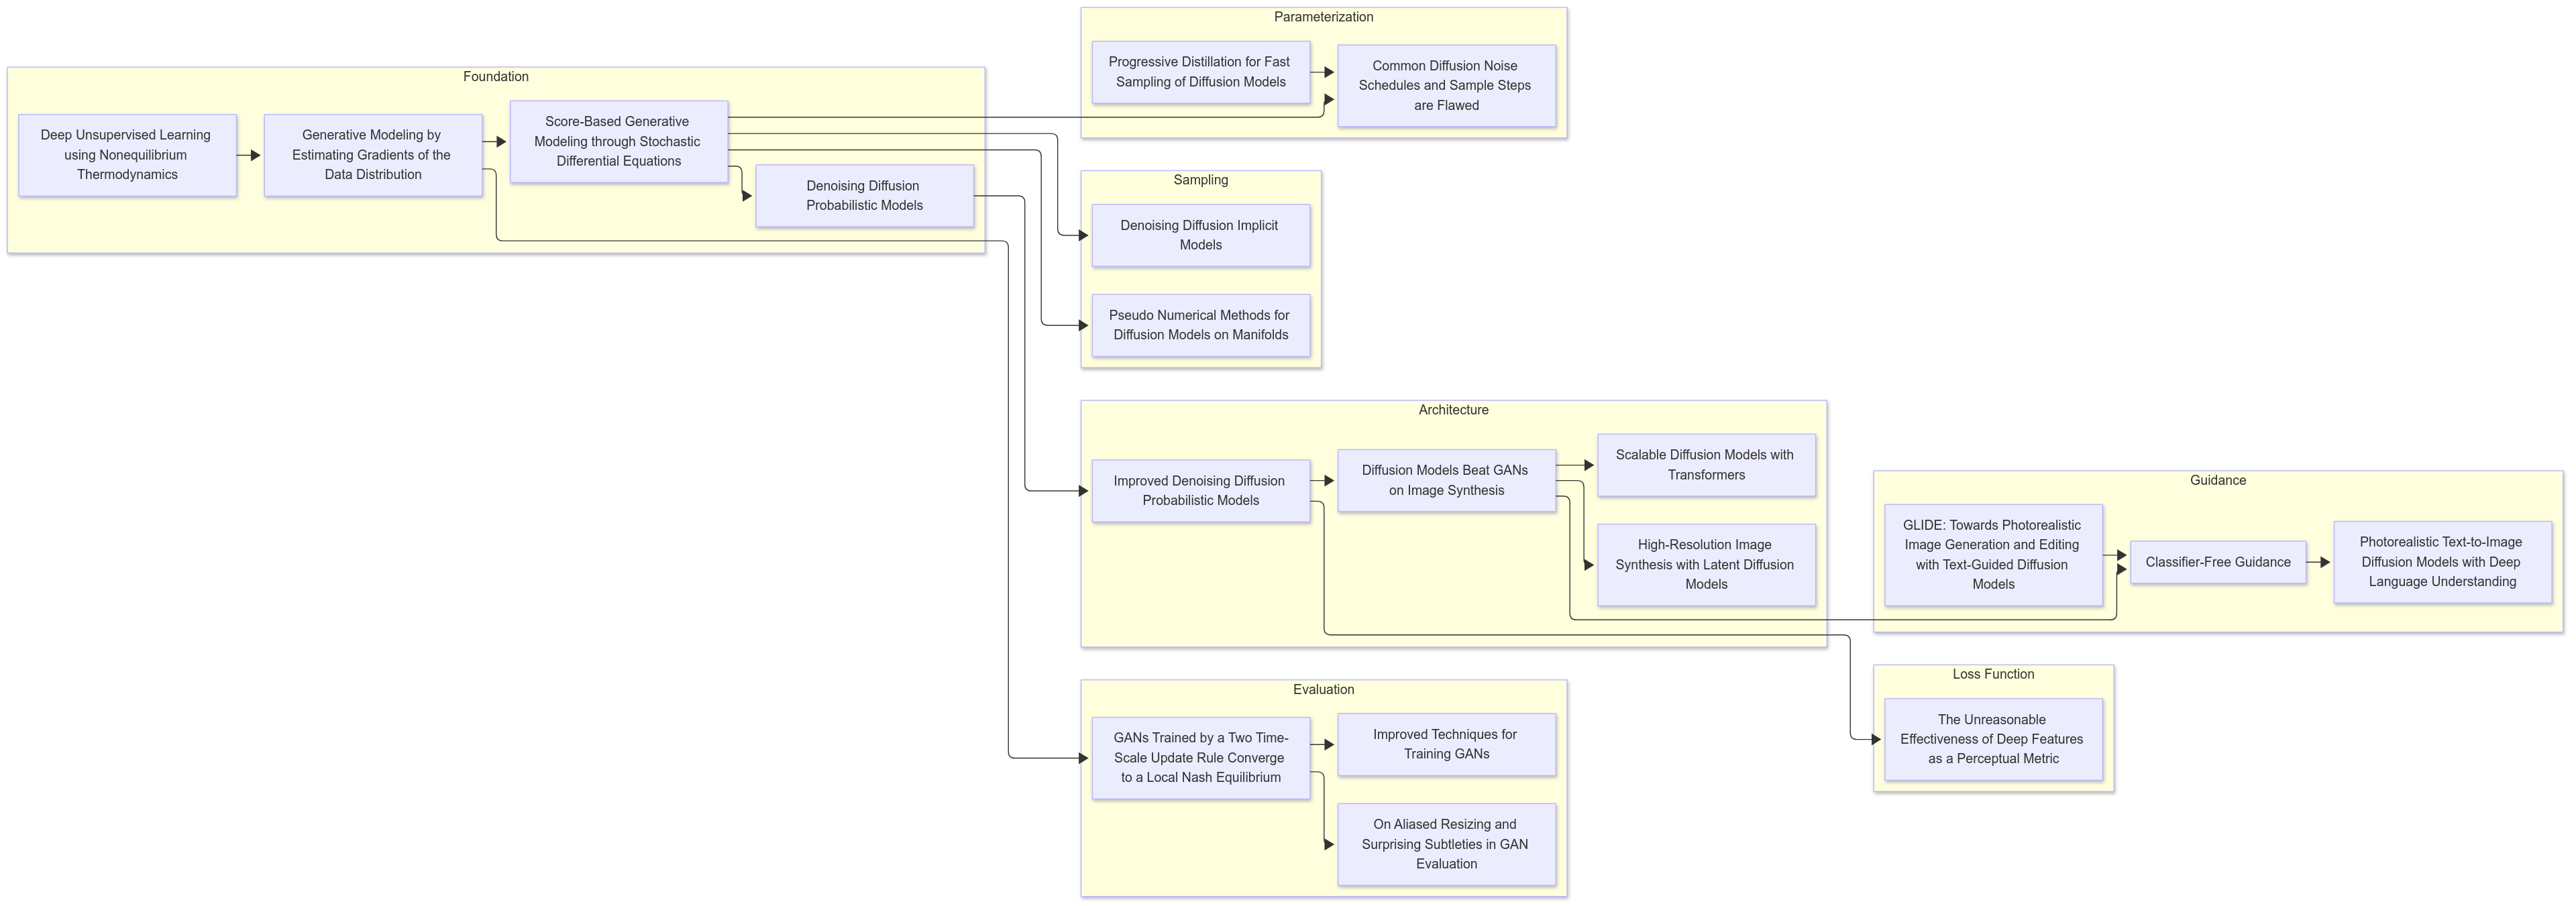
\includegraphics[width=\textwidth]{figures/figure1_mermaid.png}
    \caption{Mermaid Chart} \label{fig:fig1}
\end{figure} \FloatBarrier

\begin{figure}[H]
   \begin{minipage}{0.50\textwidth}
        \centering
        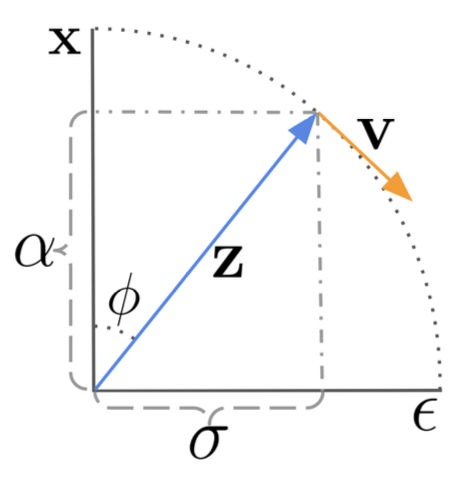
\includegraphics[width=0.7\textwidth]{figures/figure2.png}
        \caption{Parameterizing the diffusion process in terms of $\phi $ and $v_\phi$}
        \label{fig:fig2}
    \end{minipage}
    \begin{minipage}{0.50\textwidth}
        \centering
        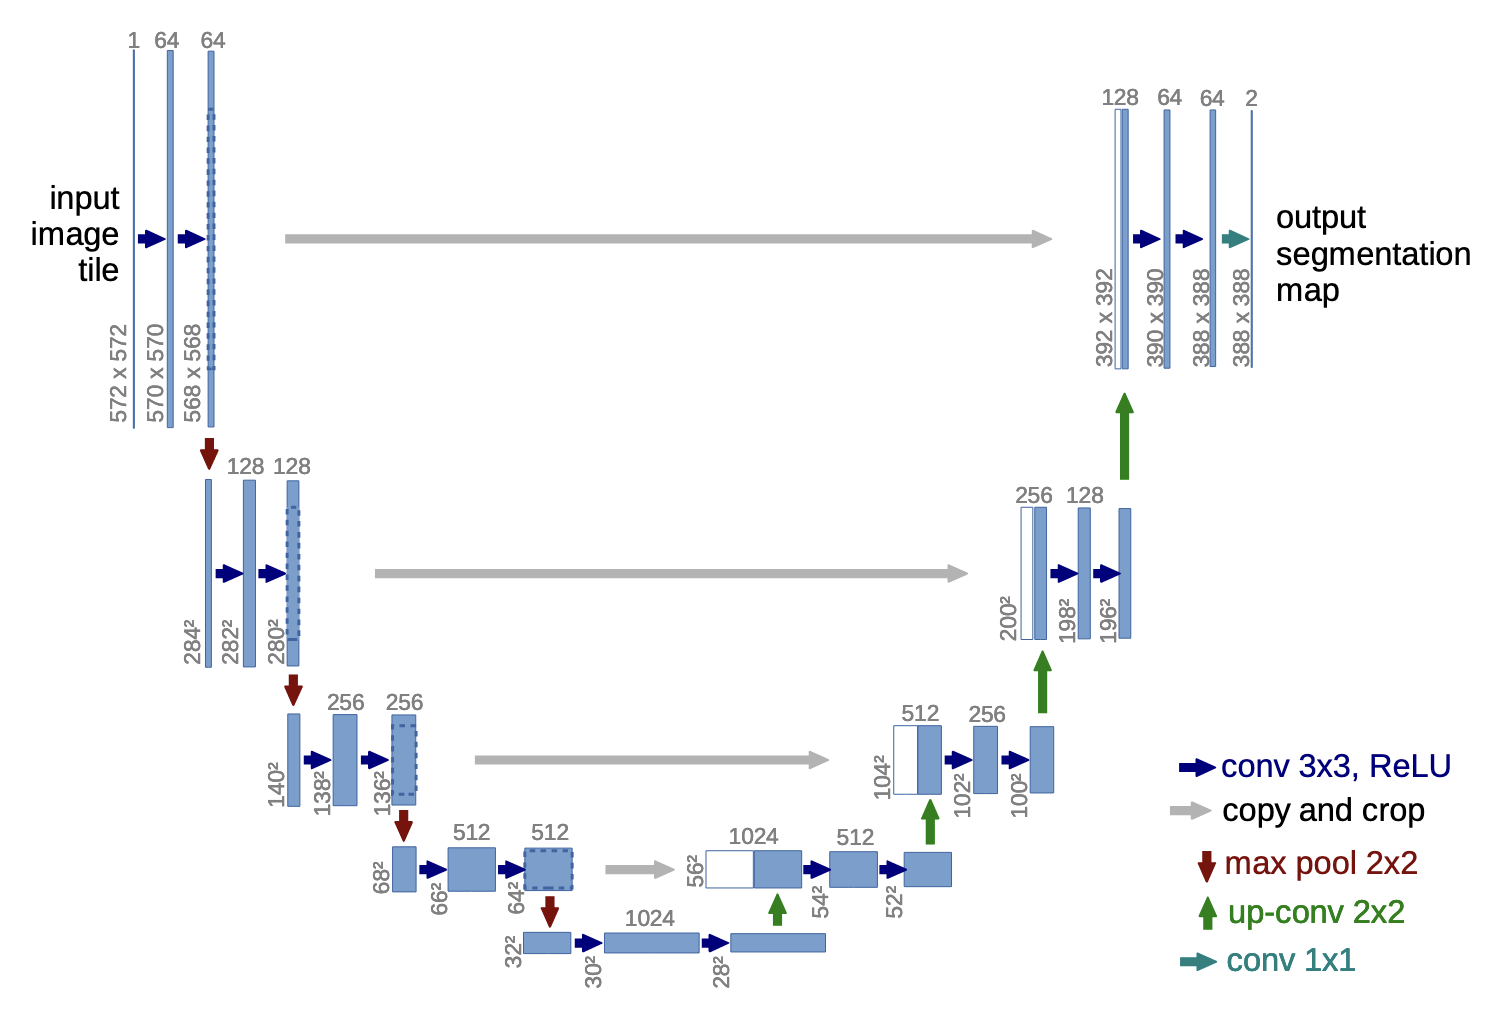
\includegraphics[width=0.9\textwidth]{figures/figure3.png}
        \caption{U-Net Architecture} \label{fig:fig3}
    \end{minipage}
\end{figure} \FloatBarrier

\begin{figure}[H]
    \begin{minipage}{0.50\textwidth}
    \centering
        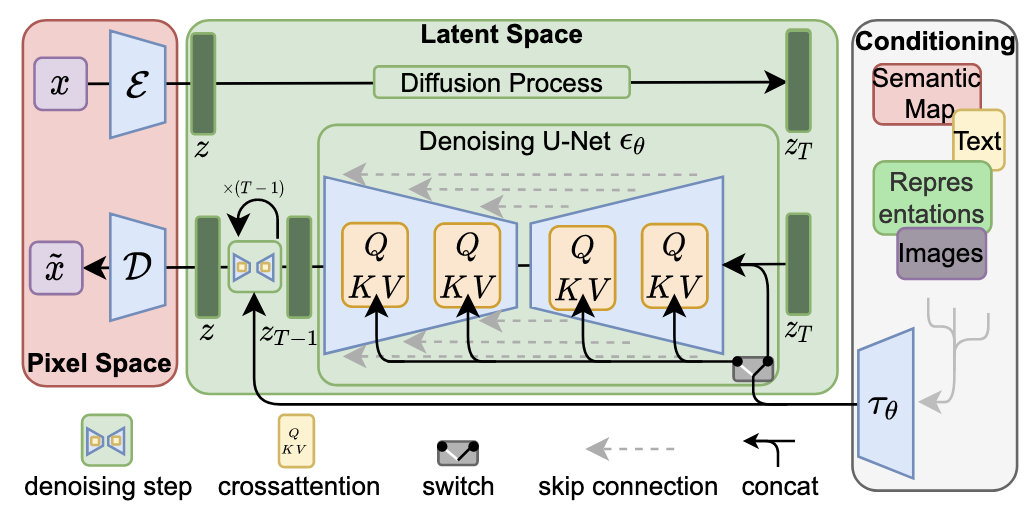
\includegraphics[width=0.9\textwidth]{figures/figure4.png}
        \caption{Latent Diffusion Model Architecture} \label{fig:fig4}
    \end{minipage}
    \begin{minipage}{0.50\textwidth}
        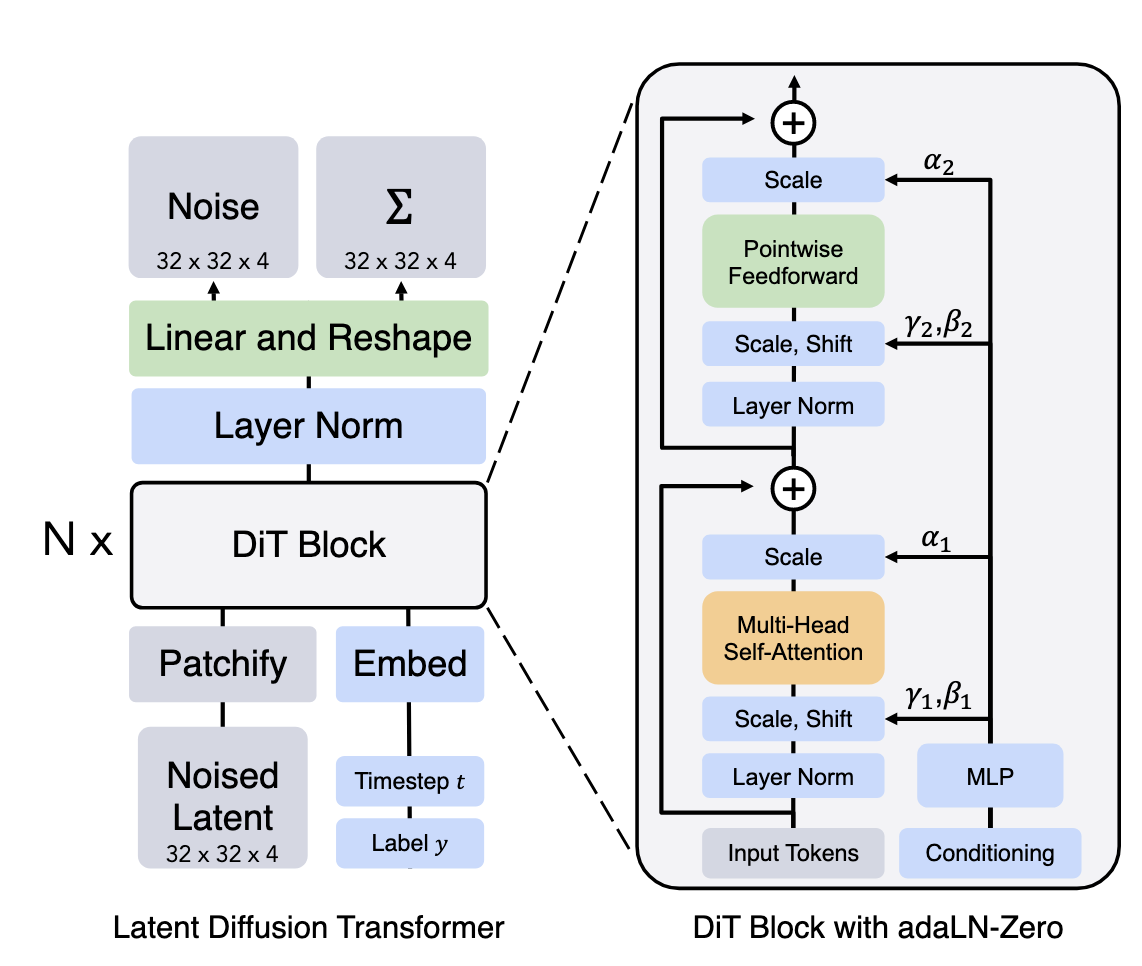
\includegraphics[width=0.9\textwidth]{figures/figure5.png}
        \caption{Diffusion Transformer Architecture} \label{fig:fig5}
    \end{minipage}
\end{figure} \FloatBarrier

\begin{figure}[H]
    \begin{minipage}{0.25\textwidth}
        \centering
        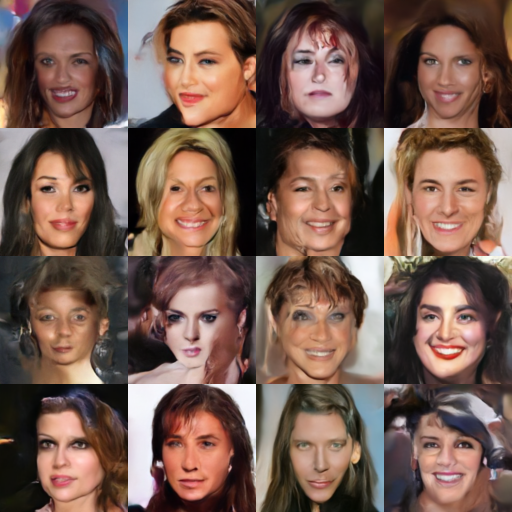
\includegraphics[width=0.9\textwidth]{figures/eta0.png}
        \caption{$\eta = 0$ (least diverse)} \label{fig:eta0}
    \end{minipage}\hfill
    \begin{minipage}{0.25\textwidth}
        \centering
        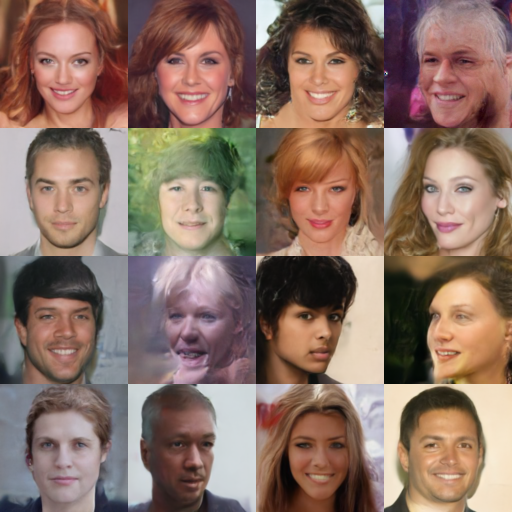
\includegraphics[width=0.9\textwidth]{figures/eta25.png}
        \caption{$\eta = 0.25$ (less  diverse)} \label{fig:eta25}
    \end{minipage}\hfill
    \begin{minipage}{0.25\textwidth}
        \centering
        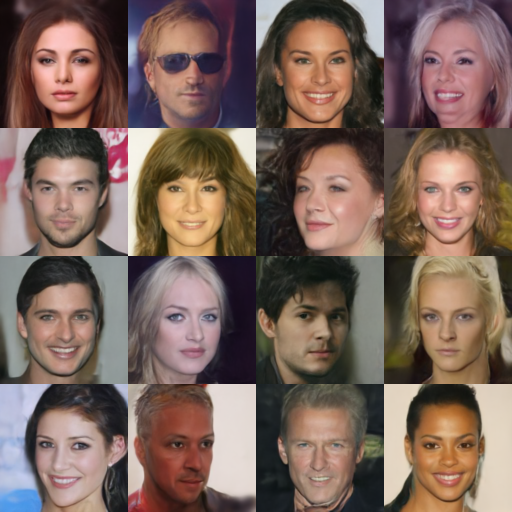
\includegraphics[width=0.9\textwidth]{figures/eta50.png}
        \caption{$\eta = 0.5$ (good balance)} \label{fig:eta50}
    \end{minipage}\hfill
    \begin{minipage}{0.25\textwidth}
        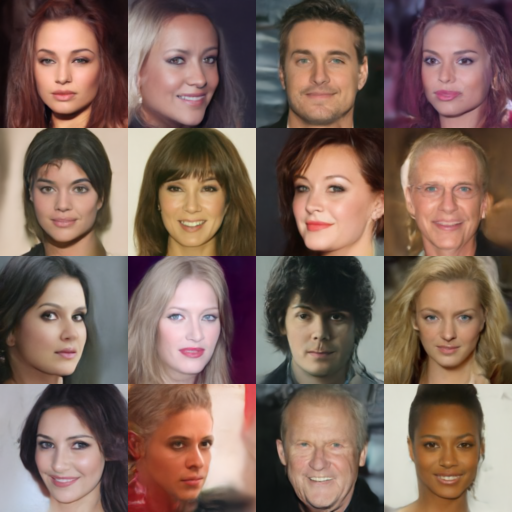
\includegraphics[width=0.9\textwidth]{figures/eta75.png}
        \caption{$\eta = 0.75$ (most diverse)} \label{fig:eta75}
    \end{minipage}
\end{figure} \FloatBarrier

\begin{figure}[H]
    \begin{minipage}{0.50\textwidth}
        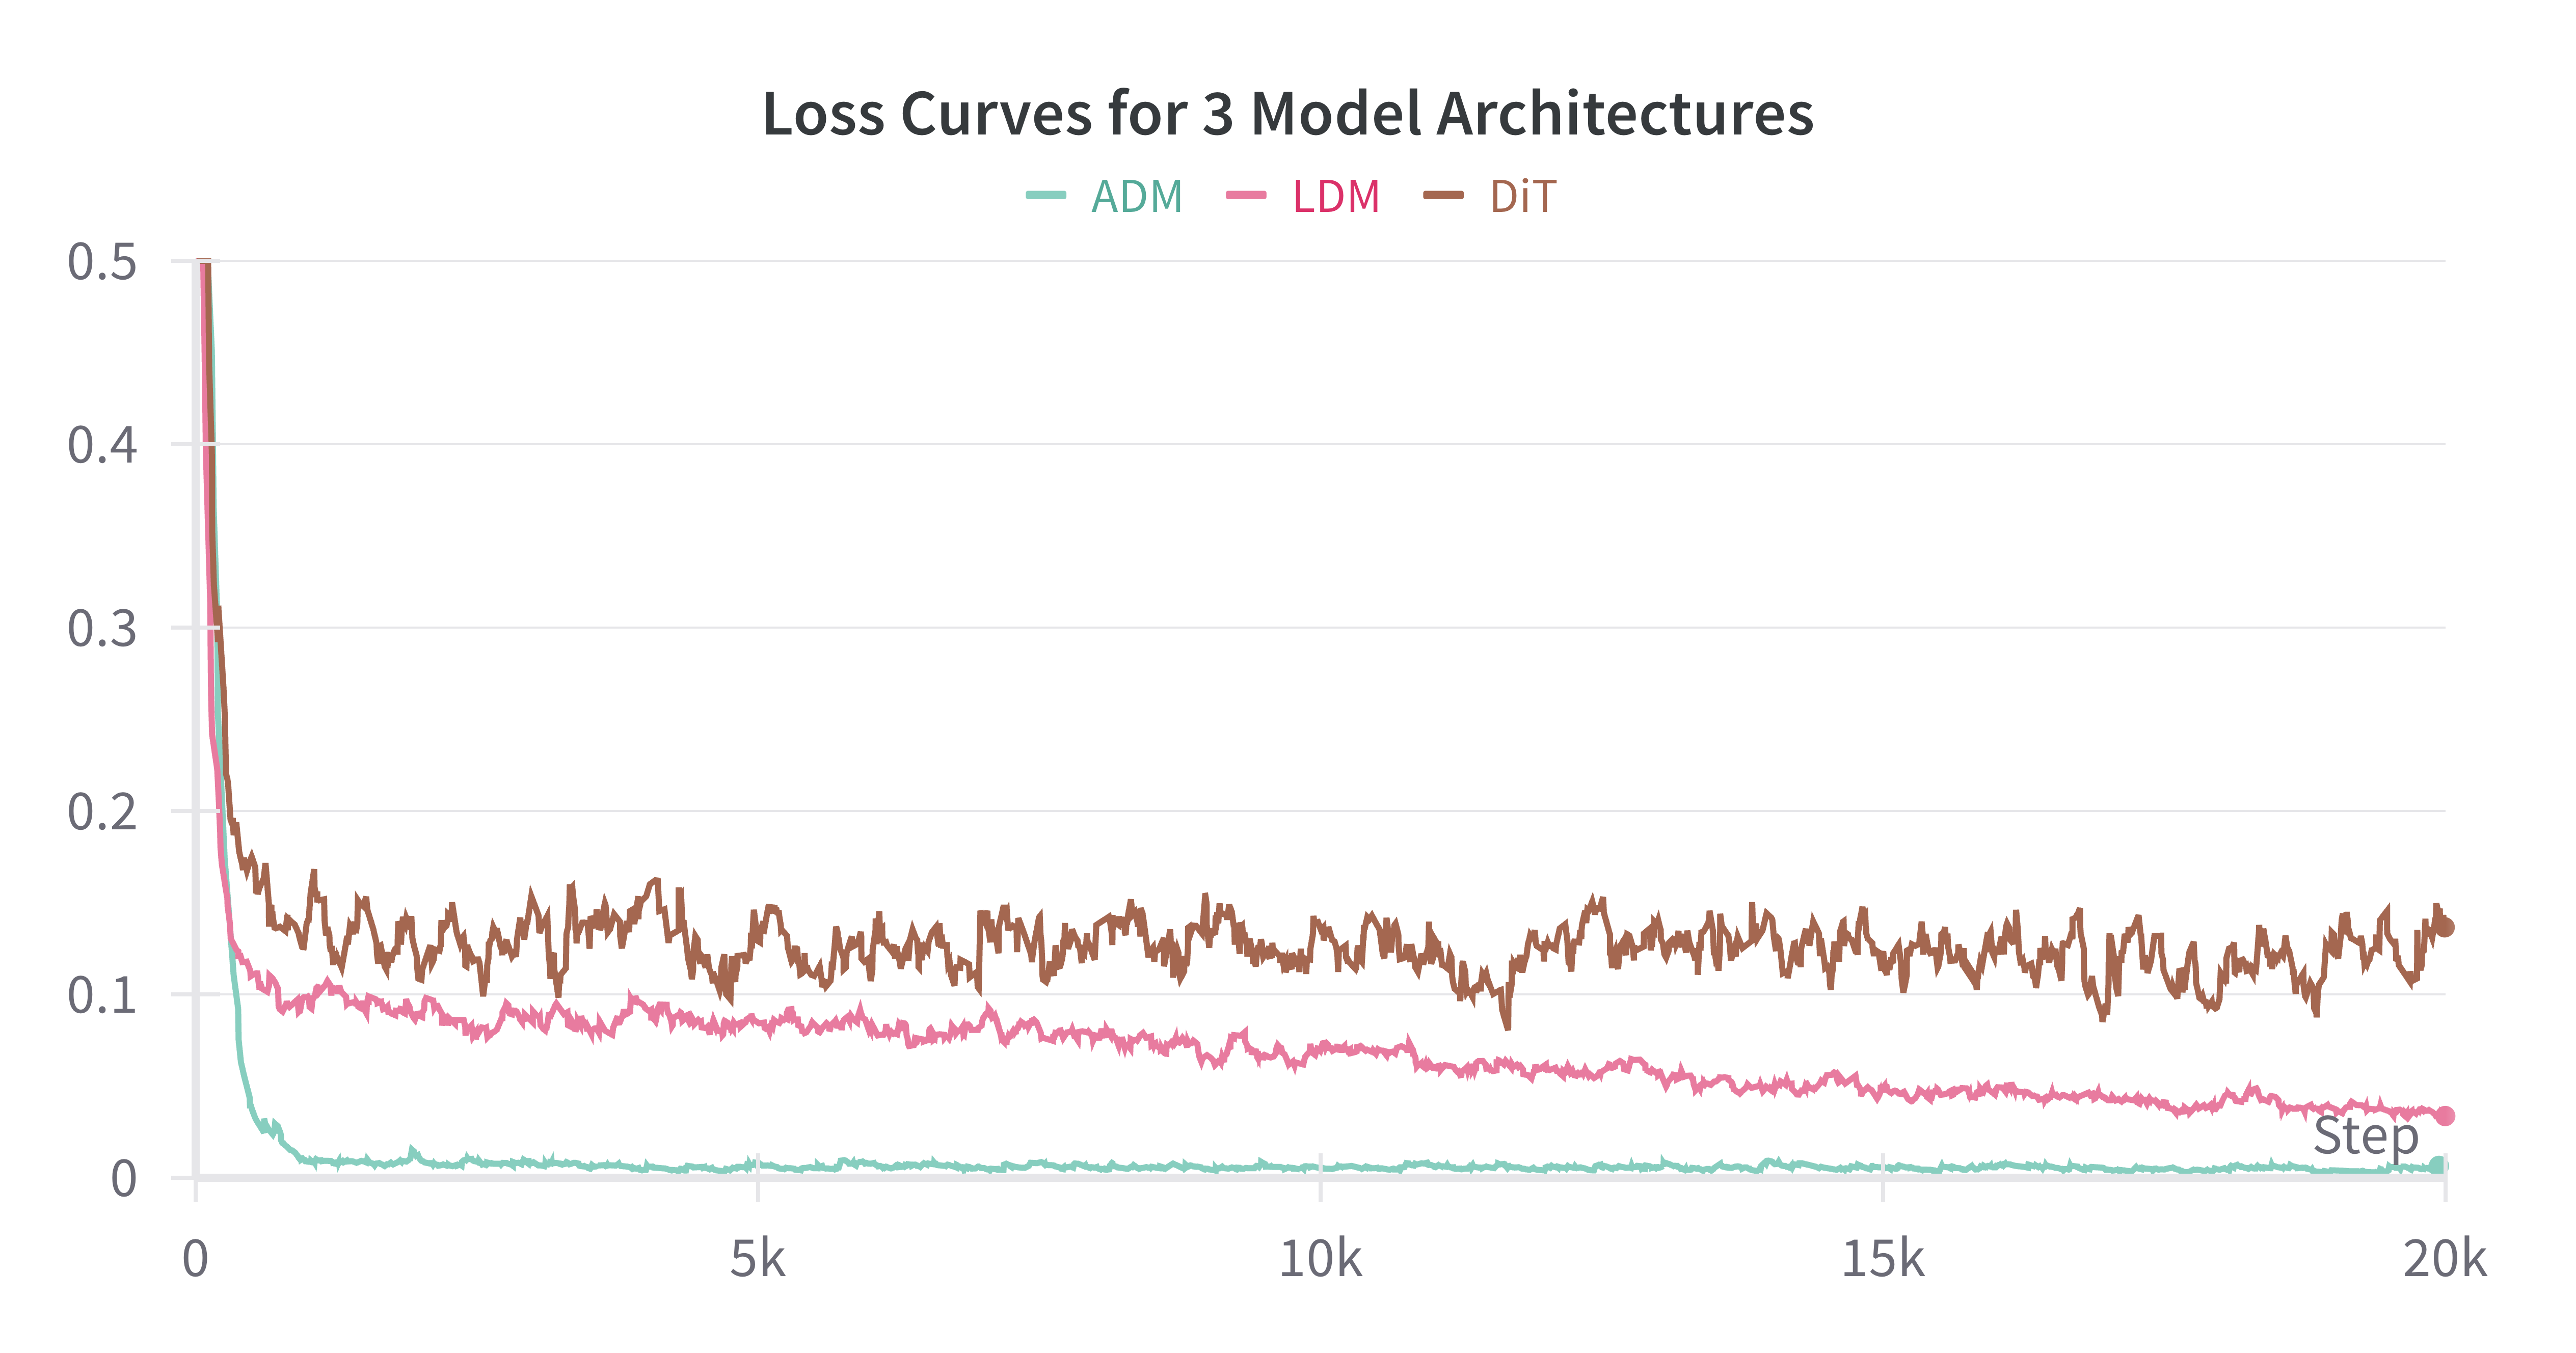
\includegraphics[width=0.9\textwidth]{figures/loss_curve3.png}
    \caption{Loss Curves for 3 Model Architectures} \label{fig:loss_architecture}
    \end{minipage}
    \begin{minipage}{0.50\textwidth}
    \centering
        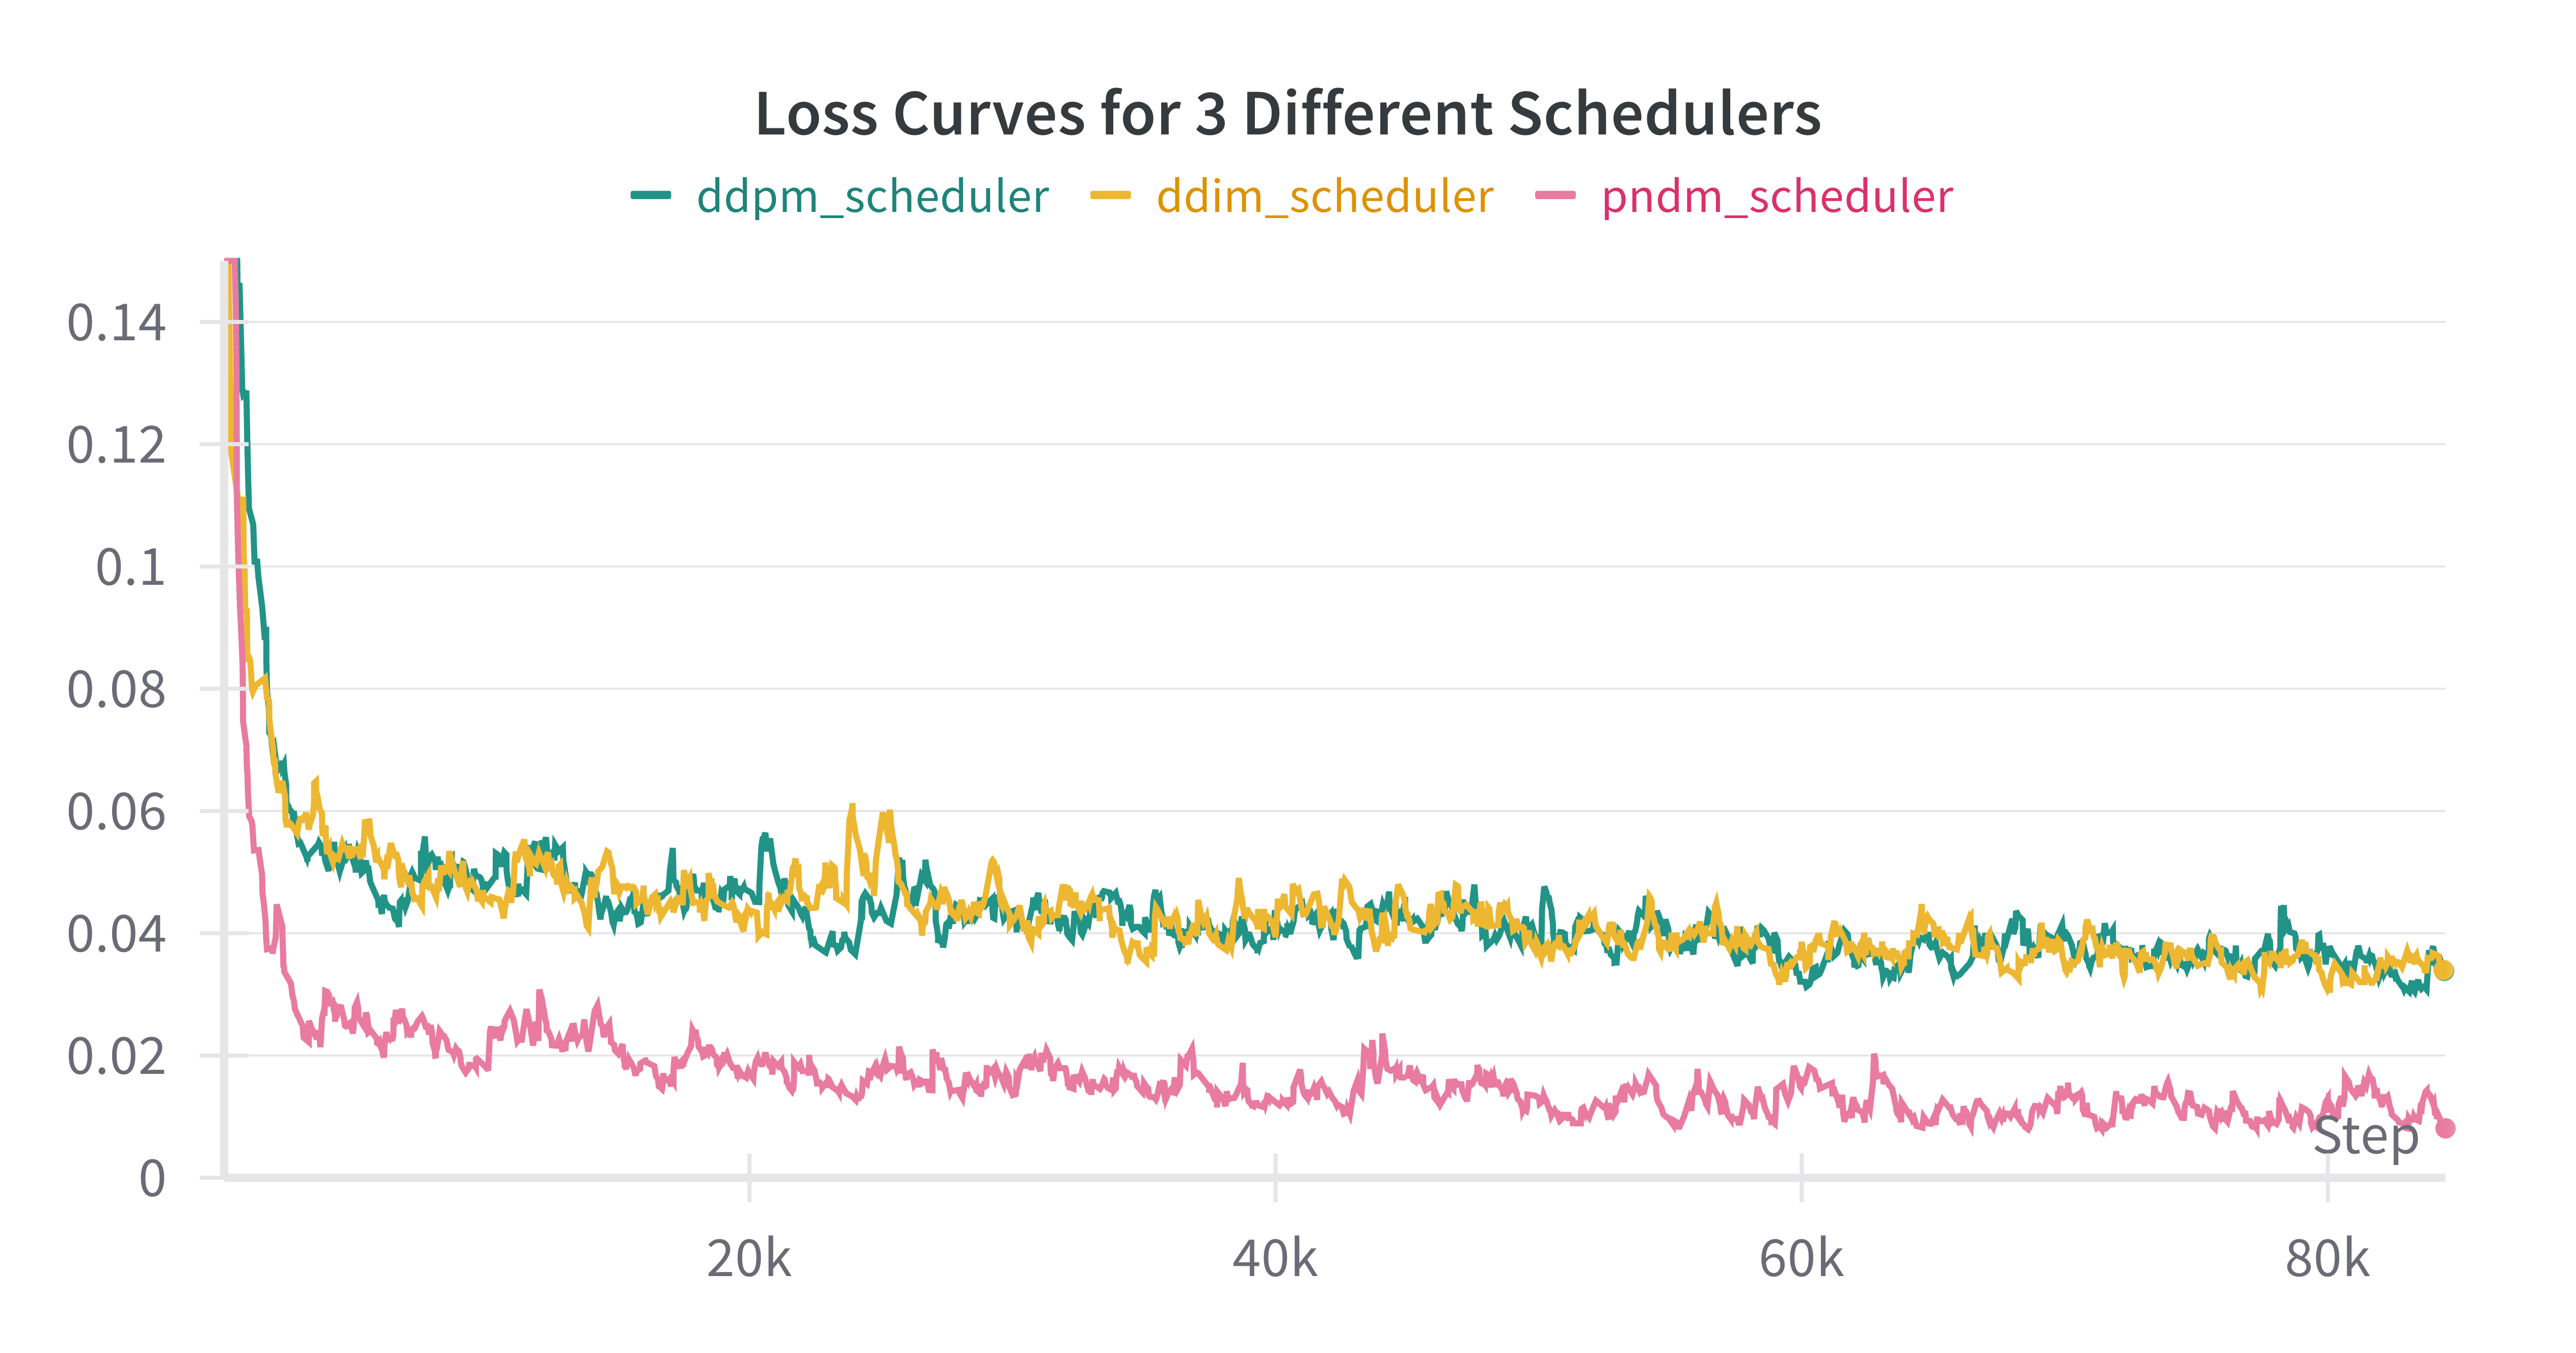
\includegraphics[width=0.9\textwidth]{figures/loss_curve2.png}
    \caption{Loss Curves for 3 Different Schedulers} \label{fig:loss_scheduler}
    \end{minipage}
\end{figure} \FloatBarrier

\begin{figure}[H]
    \begin{minipage}{0.50\textwidth}
    \centering
        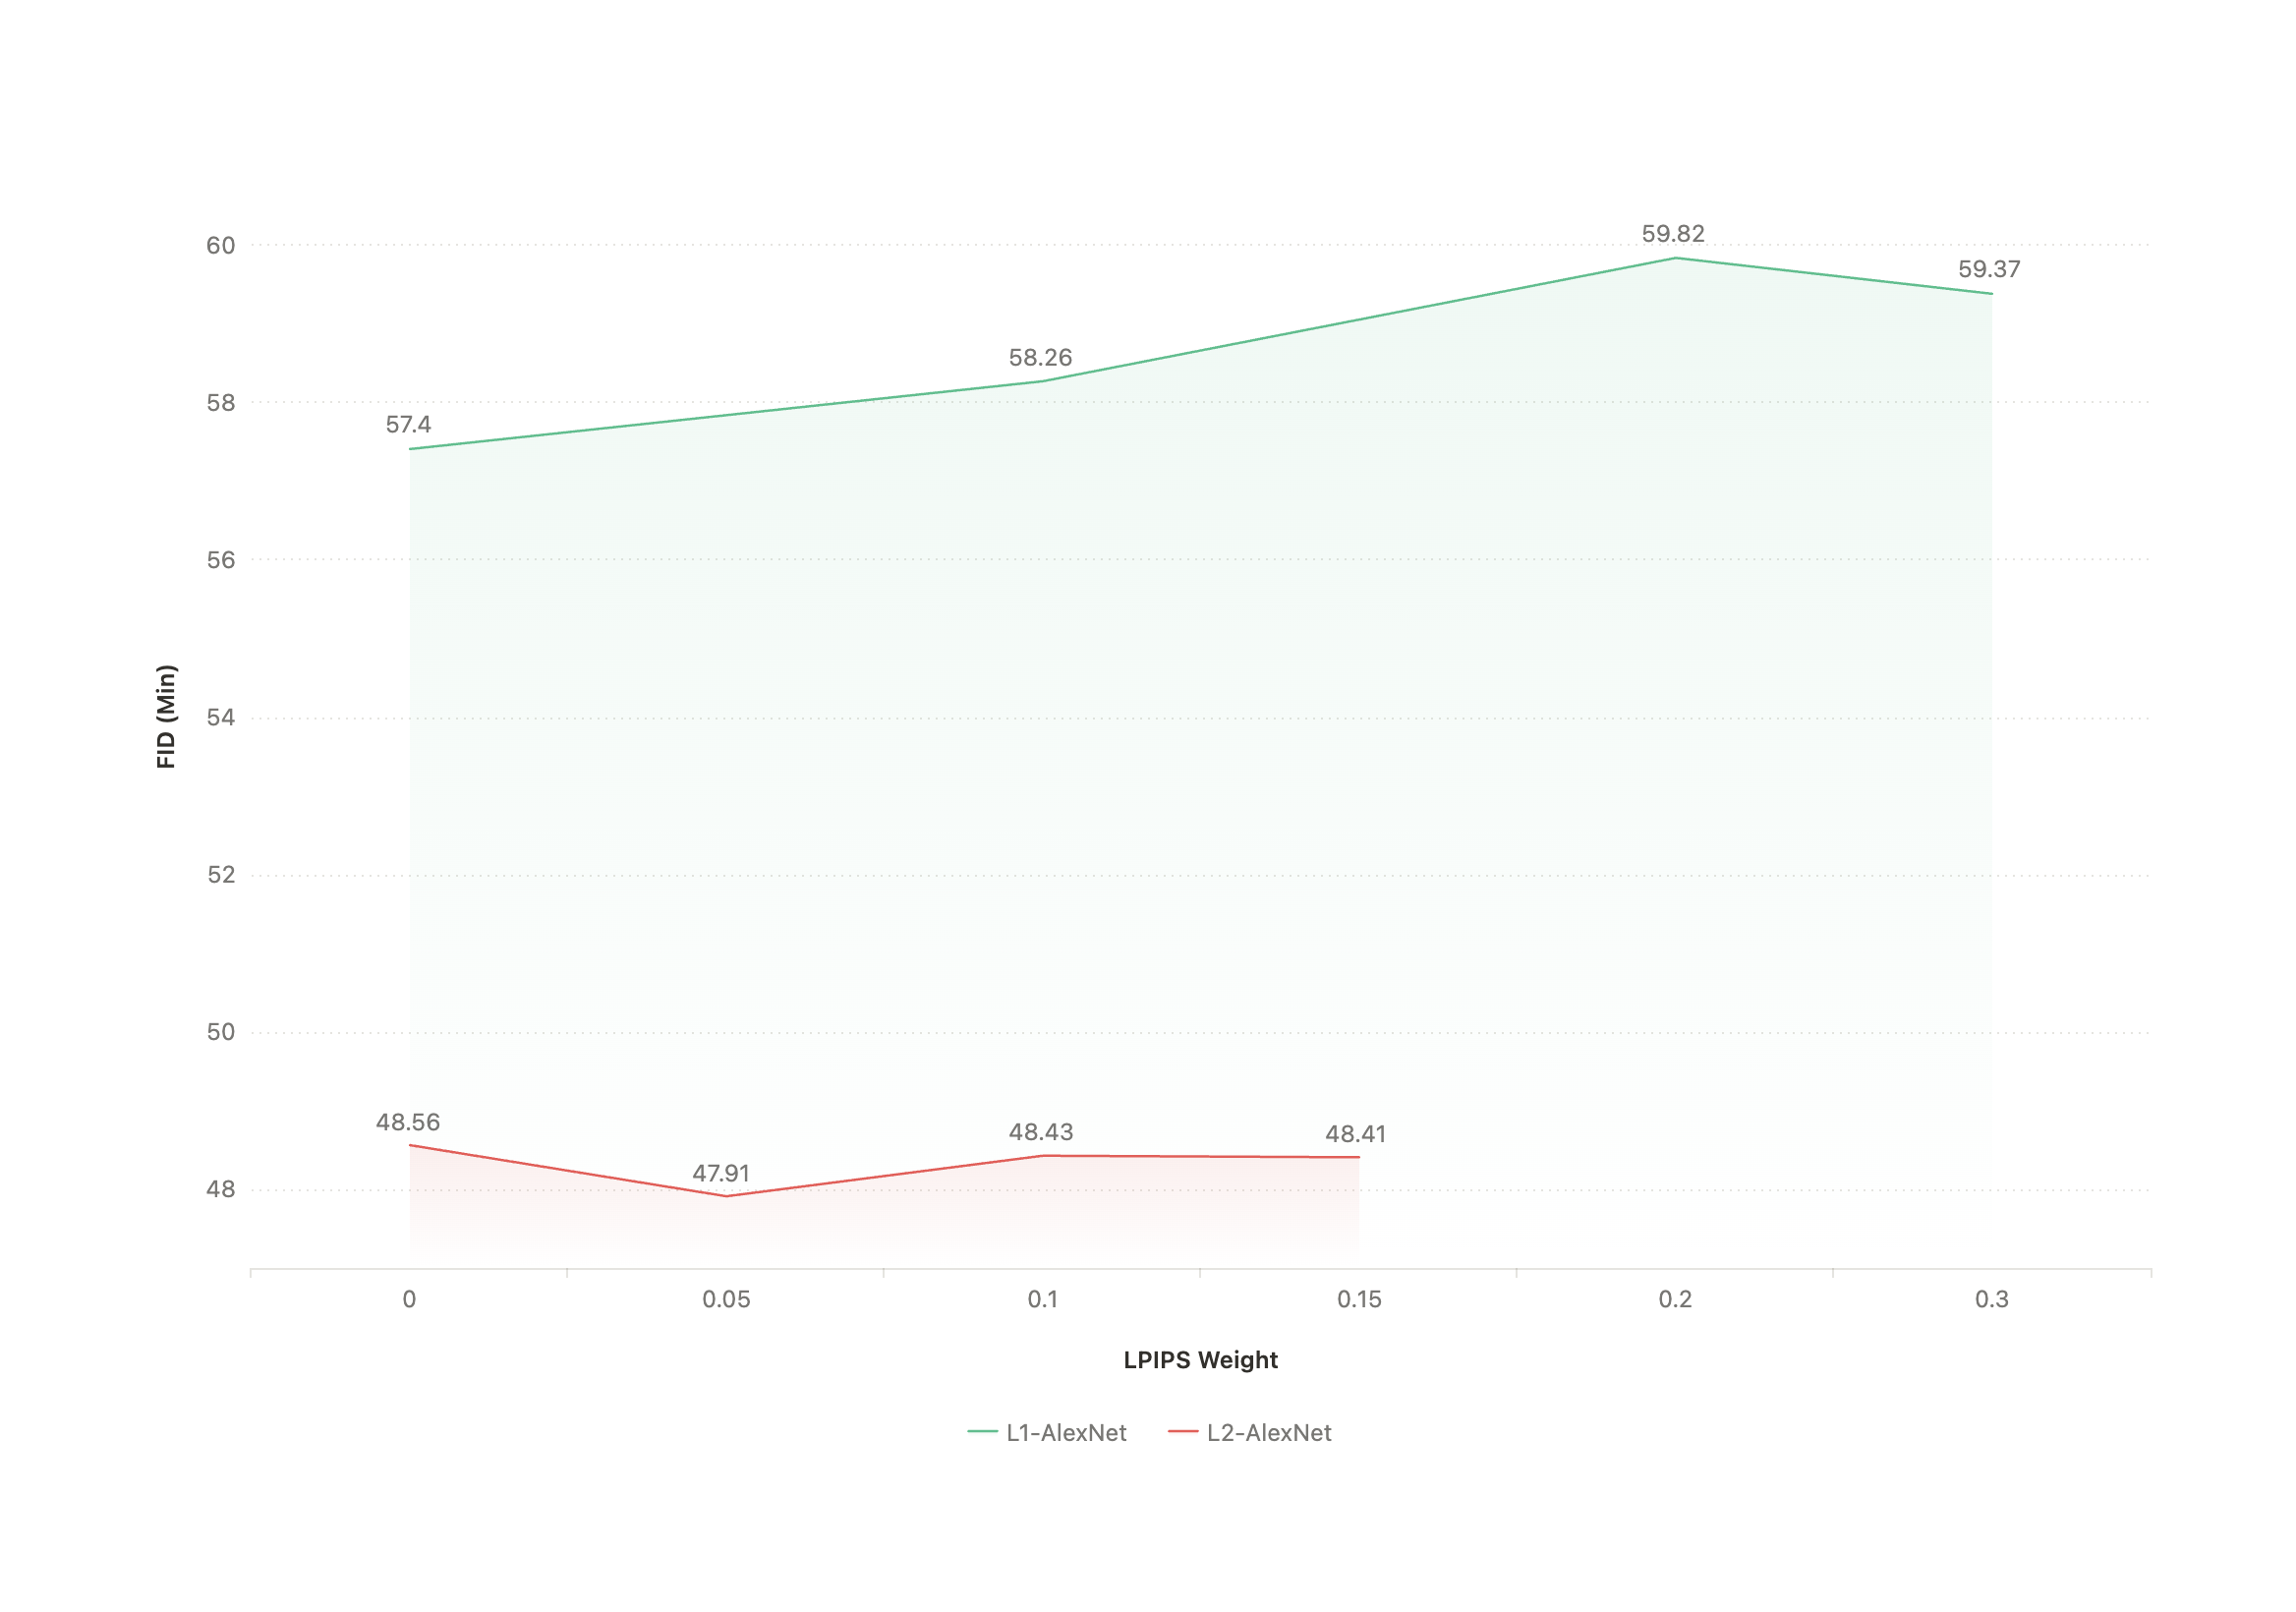
\includegraphics[width=0.9\textwidth]{figures/lpips.png}
    \caption{LPIPS Weight vs. FID} \label{fig:lpips}
    \end{minipage}
    \begin{minipage}{0.50\textwidth}
        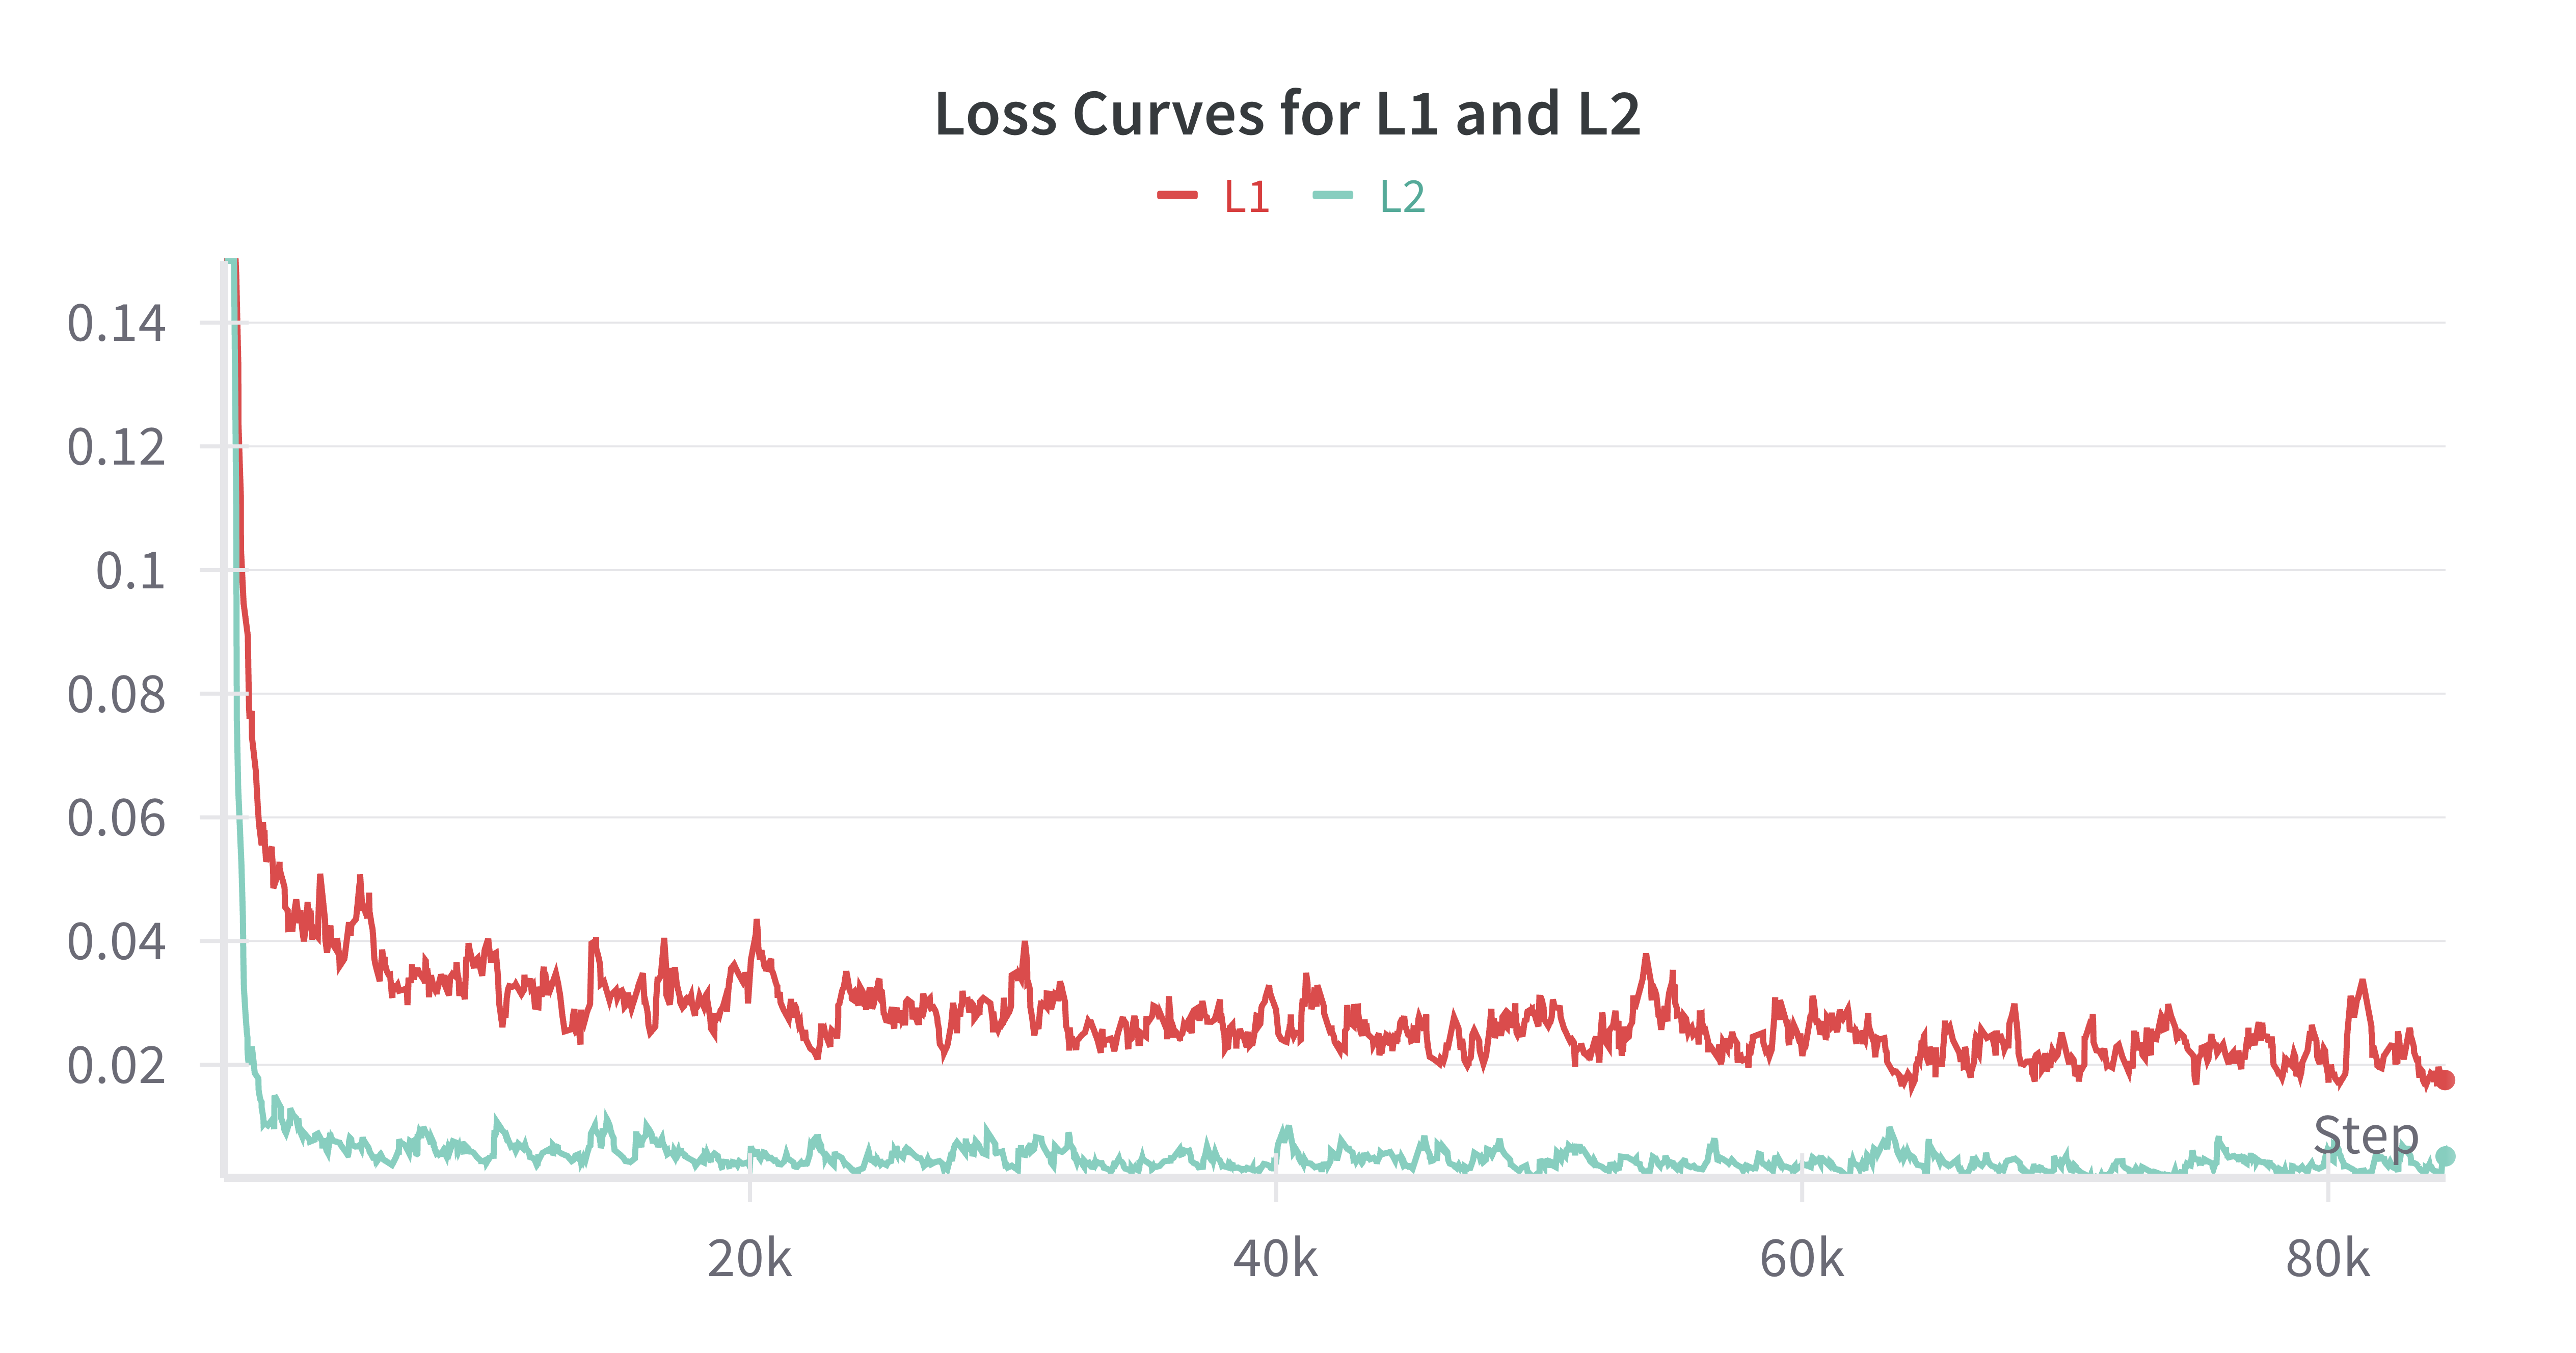
\includegraphics[width=0.9\textwidth]{figures/loss_curve.png}
    \caption{Loss Curves for L1 and L2} \label{fig:loss_l1l2}
    \end{minipage}
\end{figure} \FloatBarrier


\begin{figure}[H]
   \begin{minipage}{0.33\textwidth}
    \centering
    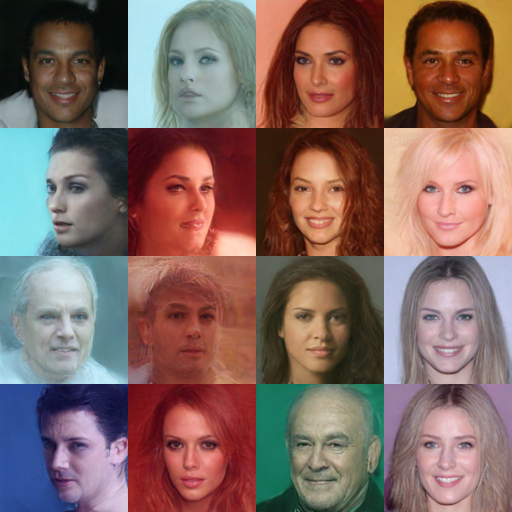
\includegraphics[width=0.9\textwidth]{figures/figure6_unconditioned.png}
    \caption{Unconditioned Output} \label{fig:unconditioned}
   \end{minipage}
   \begin{minipage}{0.33\textwidth}
    \centering
    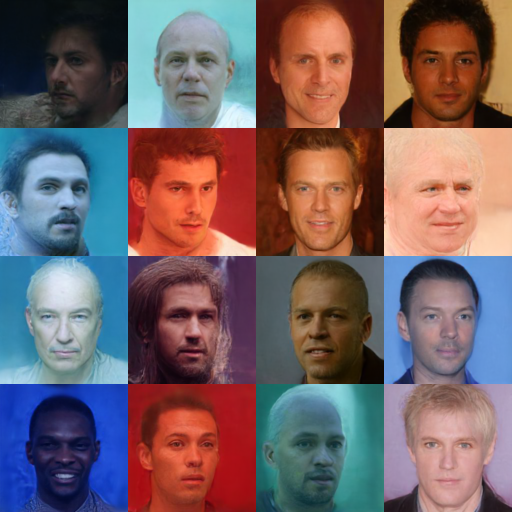
\includegraphics[width=0.9\textwidth]{figures/figure7_male_cond.png}
    \caption{Male Conditioned Output} \label{fig:male}
   \end{minipage}
   \begin{minipage}{0.33\textwidth}
    \centering
    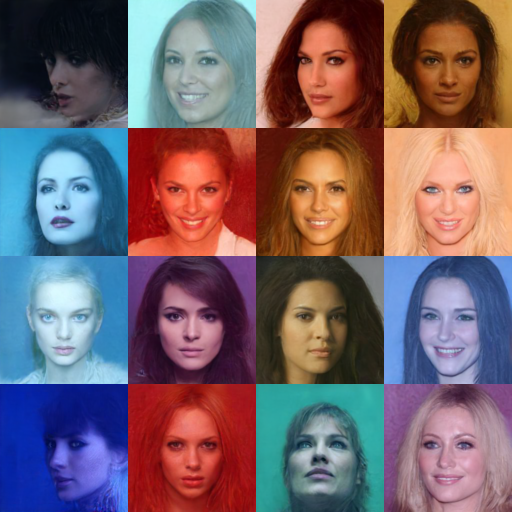
\includegraphics[width=0.9\textwidth]{figures/figure8_female_cond.png}
    \caption{Female Conditioned Output} \label{fig:female}
   \end{minipage}
\end{figure} \FloatBarrier

\begin{figure}[H]
    \begin{minipage}{0.50\textwidth}
        \centering
        \includegraphics[width=0.85\textwidth]{figures/figure9_stable-diffusion-v1-5.png}
        \caption{Fully Fine-tuned with pre-trained "stable-diffusion-v1-5" model} \label{fig:stable_diff}
    \end{minipage}
    \begin{minipage}{0.50\textwidth}
        \centering
        \includegraphics[width=0.85\textwidth]{figures/figure10_stable-diffusion-v1-5_frozen_layers.png}
        \caption{Our own fine-tuned model with the first three layers frozen} \label{fig:stable_diff_frozen}
    \end{minipage}
\end{figure}
\FloatBarrier

\subsection{Image Caption Descriptions} \label{app:image_captions}
\begin{enumerate}
    \item Portrait of a young woman with long wavy hair, soft studio lighting, high contrast, 4k resolution, professional headshot.
    \item Close-up of a smiling man with sharp jawline, cinematic lighting, shallow depth of field, bokeh background.
    \item High-fashion model with dramatic makeup, sharp cheekbones, intense gaze, in a vibrant urban setting.
    \item Natural portrait of a person with freckles, soft lighting, unretouched, authentic expression.
    \item Retro 80s style portrait, neon colors, grainy texture, bold shadows, high contrast.
    \item Black and white portrait of an elderly woman with wrinkles, deep shadows, textured background.
    \item Fashion editorial headshot, strong jawline, clean background, high key lighting, Vogue style.
    \item Glamour shot of a person with curly hair, golden hour lighting, soft focus, warm tones.
    \item Candid portrait, natural light, slight smile, outdoor background, wind-blown hair.
    \item Close-up of a person with expressive eyes, intricate makeup, glowing skin, ethereal lighting.
    \item Headshot of a person in a studio, neutral background, intense stare, perfectly lit skin.
    \item Profile shot, high-contrast lighting, dramatic shadow play, fine art portrait style.
    \item Fashion magazine cover style, high-definition, sharp details, confident expression.
    \item Editorial beauty portrait, colorful makeup, symmetrical face, close-up, glossy finish.
    \item Minimalist headshot, natural light, smooth skin texture, calm expression.
    \item Vintage portrait, faded colors, slight grain, nostalgic 70s film effect, natural hair.
\end{enumerate}
\begin{figure}[H]
   \begin{minipage}{0.50\textwidth}
    \centering
    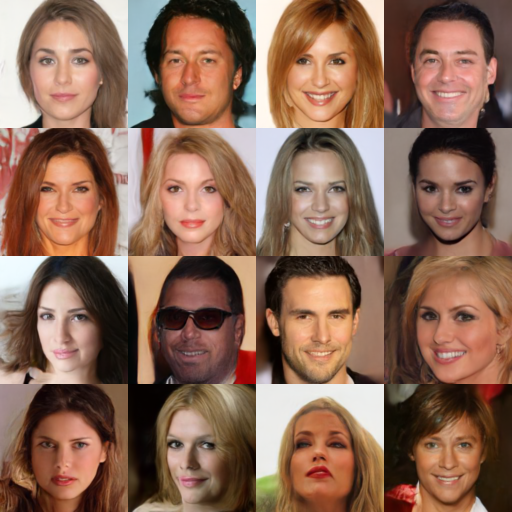
\includegraphics[width=0.85\textwidth]{figures/figure11_adm_ddpm_linear.png}
    \caption{Ablation Diffusion Model using DDPM linear schedule} \label{fig:adm_ddpm}
    \end{minipage}
       \begin{minipage}{0.50\textwidth}
        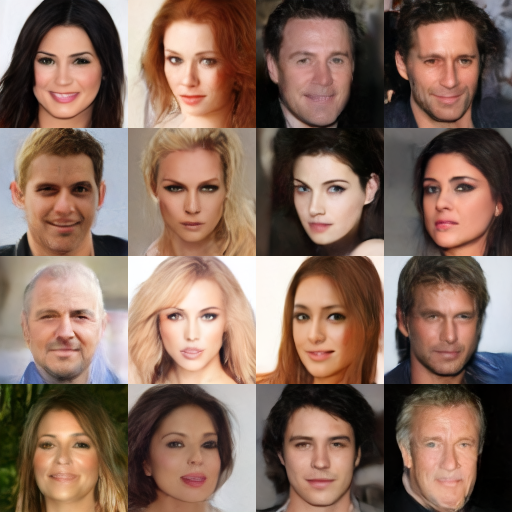
\includegraphics[width=0.85\textwidth]{figures/figure12_ldm_ddim_scaled_linear.png} \caption{Latent Diffusion Model with DDIM using scaled linear schedule} \label{fig:ldm_ddim}
    \end{minipage}
\end{figure}
\FloatBarrier
\section{Tables}



\begin{table}[H]
    \centering
    \caption{U-Net Ablation}
    \label{tab:unet_table}
    \begin{tabular}{ccccccc}
    \hline
        Channels & Depth & Heads & Attention Resolutions & BigGAN up/down sample & FID (500K) & Baseline Comparison \\ \hline
        \hline
        128 & 2 & 1 & 16 & $\times$ & 70.57 & - \\
        \hline
        128 & 4 & 1 & 16 & $\times$ & 63.84 & -6.73 \\ 
        96 & 4 & 1 & 16 & $\times$ & 69.76 & -0.81 \\ 
        64 & 4 & 1 & 16 & $\times$ & 74.72 & +4.15 \\ 
        128 & 2 & 4 & 16 & $\times$ & 63.63 & -6.94 \\ 
        128 & 2 & 1 & 32,16,8 & $\times$ & 65.07 & -5.5 \\ 
        128 & 2 & 1 & 16 & $\checkmark$ & 68.72 & -1.85 \\ 
        128 & 2 & 4 & 32,16,8 & $\checkmark$ & \textbf{62.87} & \textbf{-7.70} \\ \hline
    \end{tabular}
\end{table}

\begin{table}[H]
    \centering
    \caption{U-Net Heads Ablation}
    \label{tab:unet_heads_table}
    \begin{tabular}{ccccc}
    \hline
        \makecell{Attention\\Resolution} & Heads & \makecell{Channels \\per Head} & \makecell{FID\\ (500K)} & \makecell{Baseline\\Comparison} \\ 
        \hline
        \hline
        16 & 4 & 64 & 63.63 & - \\ 
        \hline
        16 & 2 & 128 & 63.75 & + 0.12 \\ 
        16 & 8 & 32 & \textbf{61.86} & \textbf{-1.01} \\ \hline
    \end{tabular}
\end{table}

\begin{table}[H]
    \centering
    \caption{VQ-VAE Ablation Experiments}
    \label{tab:ldm_table1}
    \begin{tabular}{cccc}
    \hline
        \makecell{Model\\Architecture} & \makecell{Commitment\\Loss Weight} & \makecell{Reconstruction\\FID} & \makecell{Baseline\\Comparison} \\
        \hline
        \hline
        VQModel & 0.1 & 30.91 & - \\
        \hline
        VQModel & 0.3 & 30.69 & -0.22 \\ 
        VQModel & 0.35 & 30.71 & -0.20 \\ 
        VQModel & 0.4 & 29.20 & -1.70 \\ 
        VQModel & 0.5 & \textbf{29.36} & \textbf{-1.55} \\ \hline
    \end{tabular}
\end{table}

\begin{table}[H]
    \centering
    \caption{LDM Model Architecture Ablation}
    \label{tab:ldm_table2}
    \begin{tabular}{cccc}
    \hline
        \makecell{Model\\Architecture} & VAE Model & FID Score & \makecell{Baseline\\Comparison} \\ \hline
        \hline
        4 Block UNet & VQ-VAE(loss-weight-0.4) & 67.05 & - \\
        \hline
        5 Block UNet & VQ-VAE(loss-weight-0.4) & 56.92 & -10.13 \\ 
        6 Block UNet & VQ-VAE(loss-weight-0.4) & 57.60 & -9.45 \\ 
        5 Block UNet & VQ-VAE(pre-train-model) & \textbf{53.35} & \textbf{-13.70} \\
        \hline
    \end{tabular}
\end{table}

\begin{table}[H]
    \centering
    \caption{VAE Architecture Ablation}
    \label{tab:dit_table1}
    \begin{tabular}{cccc}
    \hline
        Model Architecture & KL Loss Weight & Reconstruction FID & Baseline Comparison \\ \hline
        \hline
        AutoencoderKL(4 Block) & 0.5 & 69.7 & - \\
        \hline
        AutoencoderKL(4 Block) & 0.2 & 63.55 & -6.15 \\ 
        AutoencoderKL(4 Block) & 0.1 & 58.95 & -10.75 \\ 
        AutoencoderKL(4 Block) & 0.05 & 52.55 & -17.14 \\ 
        AutoencoderKL(3 Block) & 0.05 & \textbf{38.41} & \textbf{-31.29} \\ \hline
    \end{tabular}
\end{table}

\begin{table}[H]
    \centering
    \caption{DiT Model Architecture Ablation}
    \label{tab:dit_table2}
    \begin{tabular}{ccccc}
    \hline
        Model Architecture & VAE Model & Guidance Scale & FID & Baseline Comparison \\ \hline
        \hline
        DiT\_B\_2 & VAE(loss-weight-0.02) & 1 & 95.79 & - \\
        \hline
        DiT\_B\_2 & VAE(loss-weight-0.02) & 1 & 84.29 & -11.5 \\ 
        DiT\_B\_2 & VAE(loss-weight-0.1) & 4 & 84.40 & -11.39 \\ 
        DiT\_B\_2 & VAE(loss-weight-0.1) & 0 & 75.09 & -20.70 \\ 
        DiT\_B\_2 & VAE(loss-weight-0.1) & 1 & 74.38 & -21.41 \\ 
        DiT\_B\_2 & VAE(loss-weight-0.05) & 1 & \textbf{68.25} & \textbf{-27.53} \\ \hline
    \end{tabular}
\end{table}

\begin{table}[H]
    \centering
    \caption{Data Augmentation}
    \label{tab:aug_table}
    \begin{tabular}{ccc}
    \hline
        Data Augmentation & FID (500K) & Baseline Comparison \\ \hline
        \hline
        Baseline & 61.26 & - \\ 
        \hline
        Center Crop & 51.69 & -9.57 \\ 
        Random Horizontal Flip & 49.63 & -11.62 \\ 
        Gaussian Blur & 52.66 & -8.59 \\ 
        Random Horizontal Flip + Gaussian Blur & 52.24 & -9.01 \\ 
        Random Horizontal Flip + Center Crop & 49.62 & -11.64 \\ 
        Random Horizontal Flip + Center Crop (4K Steps) & \textbf{48.32} & \textbf{-12.94} \\ \hline
    \end{tabular}
\end{table}

\begin{table}[H]
    \centering
    \caption{Training Steps vs. FID for DDPM}
    \label{tab:scheduler_table}
    \begin{tabular}{ccc}
    \hline
        Scheduler & Training Steps & FID \\
        \hline
        \hline
        DDPM & 1000 & 61.26 \\
        \hline
        DDPM & 2000 & 52.76 \\ 
        DDPM & \textbf{4000} & \textbf{48.56} \\ \hline
    \end{tabular}
\end{table}

\begin{table}[H]
    \centering
    \caption{Beta Schedule vs. FID}
    \label{tab:scheduler_table2}
    \begin{tabular}{ccccc}
    \hline
        Scheduler & Beta Schedule & Training Steps & FID & Baseline Comparison \\
        \hline
        \hline
        DDPM & \textbf{Linear} & 1000 & \textbf{61.26} & - \\
        \hline
        DDPM & Scaled Linear & 1000 & 67.04 & 5.79 \\ 
        DDPM & Cosine & 1000 & 70.70 & 9.46 \\ \hline
    \end{tabular}
\end{table}

\begin{table}[H]
    \centering
    \caption{DDIM Beta Schedule vs. FID}
    \label{tab:scheduler_table3}
    \begin{tabular}{ccccc}
    \hline
        Scheduler & Beta Schedule & Inference Steps & FID & Baseline Comparison \\ \hline
        \hline
        DDIM & Linear & 100 & 59.94 & - \\ 
        \hline
        DDIM & Scaled Linear & 100 & 55.77 & -4.16 \\ 
        DDIM & Cosine & 100 & \textbf{52.63} & \textbf{-7.30} \\ \hline
    \end{tabular}
\end{table}

\begin{table}[H]
    \centering
    \caption{PNDM Beta Schedule vs. FID}
    \label{tab:scheduler_table4}
    \begin{tabular}{ccccc}
    \hline
        Scheduler & Beta Schedule & Inference Steps & FID & Baseline Comparison \\
        \hline   
        \hline
        PNDM & \textbf{Linear} & 50 & \textbf{56.79} & - \\
        \hline
        PNDM & Scaled Linear & 50 & 58.25 & 1.46 \\ 
        PNDM & Cosine & 50 & 71.12 & 14.33 \\ \hline
    \end{tabular}
\end{table}

\begin{table}[H]
    \centering
    \caption{$\eta$ vs. FID}
    \label{tab:scheduler_table5}
    \begin{tabular}{ccccc}
    \hline
        $\eta$ & FID & IS & Baseline FID Comparison \\
        \hline   
        \hline
        0.0 (baseline) & 52.63 & 2.40 ± 0.22 & - \\
        \hline
        0.25 & 55.3 & 2.33 ± 0.17 & 2.67 \\ 
        0.5 & \textbf{50.8} & \textbf{2.29 ± 0.22} & \textbf{-1.83} \\ 
        0.75 & 52.19 & 2.27 ± 0.32 & -0.51 \\ \hline
    \end{tabular}
\end{table}

\begin{table}[H]
    \centering
    \caption{Prediction Type and Zero SNR vs. FID}
    \label{tab:scheduler_table6}
    \begin{tabular}{ccccc}
    \hline
        Pipeline & Prediction Type & Zero SNR & FID (500K) & Baseline FID Comparison \\
        \hline
        \hline
        DDIM  & $\epsilon$ & No & 52.63 & - \\
        \hline
        DDIM & $v$ & Yes & \textbf{49.83} & \textbf{-2.80} \\ \hline
    \end{tabular}
\end{table}

\begin{table}[!ht]
    \centering
    \caption{Loss Function vs. FID}
    \label{tab:loss_table}
    \begin{tabular}{ccccccc}
    \hline
        Loss Function & LPIPS Enabled & LPIPS Network & LPIPS Weight & FID (500K) & Run Time & Baseline Comparison \\ \hline
        \hline
        L2 & No & - & 0 & 48.56 & 15h 23m 34s & - \\
        \hline
        L2 & Yes & VGG-16 & 0.1 & 49.23 & 15h 11m 51s & 0.67 \\ 
        L2 & Yes & AlexNet & 0.1 & \textbf{48.43} & 14h 56m 27s & \textbf{-0.13} \\ 
        L1 & No & - & 0 & 57.4 & 15h 25m 8s & 8.84 \\ 
        L1 & Yes & VGG-16 & 0.1 & 59.84 & 14h 46m 28s & 11.28 \\ 
        L1 & Yes & AlexNet & 0.1 & 58.26 & 14h 58m 11s & 9.70 \\ \hline
    \end{tabular}
\end{table}

\begin{table}[H]
    \centering
    \caption{Conditioning On Male vs. Female Label}
    \label{tab:conditioning_table}
    \begin{tabular}{cccc}  
    \hline
        Condition & Guidance Scale & IS & FID (500K) \\
        \hline
        \hline
        None & - & 2.08& 62.87 \\ 
        \hline
        Male & 0.5 & 2.14& 70.78 \\ 
        Female & 0.5 & 2.17 & 83.37 \\ \hline
    \end{tabular}
\end{table}

\begin{table}[H]
    \centering
    \caption{Contribution Table}
    \label{tab:conditioning_table}
    \begin{tabular}{|c|c|c|}  
    \hline
        \textbf{Group Member} & \textbf{Contribution Score} & \textbf{Description}\\
        \hline
        \hline
        Frank Lu & \textbf{32} & \makecell{I completed the literature review section and was responsible for\\overall project management, planning, and task delegation. I also\\conducted architecture ablation experiments and designed the\\layout for all experiments. Additionally, I fine-tuned a LoRA Stable\\Diffusion model and implemented classifier-free guidance. I\\refactored and maintained the majority of the codebase while\\reviewing pull requests from other teammates. } \\ \hline
        Kaan Emre Sanal & \textbf{18} & \makecell{I contributed to args.py and handled the Sections III.B, IV.B.1, and\\IV.B.2. I ran several experiments and handled most of the LaTeX\\documentation. I acknowledge that my contributions were\\limited. My coding skills need improvement, and I faced\\challenges due to falling behind on lectures and experiencing\\a hectic Easter break.} \\ \hline
        Ziyu Wang & \textbf{18} & \makecell{I mainly completed the sections on DDIM, v-prediction and zero\\SNR in hyperparameter tuning, as well as the loss function\\section. My contribution was limited due to gaps in my\\fundamental knowledge and practical skills regarding diffusion\\coding. } \\ \hline
        Xiaoguang Liang & \textbf{32} & \makecell{I primarily authored the literature review section, the LDM and\\DiT components of the methodology section, and conducted\\experiments with LDM, DiT, and Stable Diffusion. I also\\contributed to developing the core functionality of the project.} \\
        \hline
    \end{tabular}
\end{table}


\end{document} 
